\documentclass[12pt]{report}
\usepackage[utf8]{inputenc}
\usepackage{natbib}%referencing
\usepackage[left=1.0in,right=1.0in,top=.8in,bottom=.8in]{geometry}
\usepackage{float}
\linespread{1.3}
\usepackage{graphicx}%figures
\usepackage{geometry}
\usepackage{amsmath}%math
\usepackage{pgfplots}
\usepackage{tikz}
\usepackage{pgf-pie}
\usepackage{pdfpages}
\usepackage{textcase}
\usepackage{caption}
\pgfplotsset{width=15cm,compat=1.9}

\usepackage{titlesec} %formatting chapters
%\titlespacing*{<command>}{<left>}{<before-sep>}{<after-sep>}
\titlespacing*{\chapter}{-15pt}{10pt}{15pt}
\titlespacing*{\section}{0pt}{0pt}{5pt}
\titlespacing*{\subsection}{0pt}{5pt}{5pt}
\titleformat{\chapter}[hang] 
{\normalfont\huge\bfseries}{\chaptertitlename\ \thechapter.}{1em}{}
\renewcommand{\chaptername}{}
\graphicspath{{Images/}}%image folder name
%Cover page contents
\title{
{
\includegraphics[scale=.3]{logotu.jpg}}\\
\uppercase{\large{
    {Tribhuvan University}\\
    {Institute of Engineering}\\
    {Pulchowk Campus}\\
    \vspace{.5cm}
    {A Project Report\\ On\\Keyphrase Detection and Question Generation from Text using Machine Learning}\\
    \vspace{.5cm}
    {\textbf{Submitted By:}\\Aayush Lamichhane (PUL075BCT005) \\
    Bishal Katuwal (PUL075BCT028) \\
    Bishant Baniya (PUL075BCT030) \\
    Gobind Pd Sah (PUL075BCT038) }\\
    \vspace{.5cm}
    {\textbf{Submitted To:}\\ Department of Electronics \& Computer engineering}
    }
    \date{A\MakeLowercase{pril}, 2023}
    }
    }
\begin{document}
\maketitle
\pagenumbering{roman}
\newgeometry{top = 5cm}
\chapter*{Page of Approval}
\addcontentsline{toc}{chapter}{\numberline{}Page of Approval}
% \vspace{0.3cm}
The undersigned certifies that they have read and recommended to the Institute of Engineering for acceptance of a project report entitled \textbf{"Keyphrase Detection and Question Generation from Text using Machine Learning"} submitted by \textbf{Aayush Lamichhane}, \textbf{Bishal Katuwal}, \textbf{Bishant Baniya}, \textbf{Gobind Prasad Sah} in partial fulfillment of the requirements for the Bachelor's degree in Electronics \& Computer Engineering.\\
\vspace{1cm}\\
\begin{minipage}{.5\textwidth}
        \raggedright
    .............................\\
    Supervisor\\
    \textbf{Er. Santosh Giri}\\
    Assistant Professor\\
    Department of Electronics and Computer Engineering,\\
    Pulchowk Campus, IOE, TU.\\
    \end{minipage}%
    \begin{minipage}{0.5\textwidth}
    \raggedleft
    .............................\\
    External examiner\\
    \textbf{Anjesh Tuladhar}\\
    Chief Executive Officer\\
    Bhoos Entertainment,\\
    Jwagal, Lalitpur, Nepal.\\
    \end{minipage}\\
    \vspace{.6cm}
    \begin{center}
    .............................\\
    Head of Department\\
    \textbf{Dr. Jyoti Tandukar}\\
    Associate Professor\\
    Department of Electronics and Computer Engineering,\\
    Pulchowk Campus, IOE, TU.\\
    \vspace{.4cm}
    \end{center}

\centerline{Date of approval: June 26, 2023}
%new chapter
\restoregeometry
\chapter*{Copyright}
\addcontentsline{toc}{chapter}{\numberline{}Copyright}
The author has agreed that the Library, Department of Electronics and Computer Engineering, Pulchowk Campus, Institute of Engineering may make this report freely available for inspection. Moreover, the author has agreed that permission for extensive copying of this project report for scholarly purposes may be granted by the supervisors who supervised the project work recorded herein or, in their absence, by the Head of the Department wherein the project report was done. It is understood that the recognition will be given to the author of this report and to the Department of Electronics and Computer Engineering, Pulchowk Campus, Institute of Engineering in any use of the material of this project report. Copying or publication or the other use of this report for financial gain without approval of to the Department of Electronics and Computer Engineering, Pulchowk Campus, Institute of Engineering and author's written permission is prohibited.\\
Request for permission to copy or to make any other use of the material in this report in whole or in part should be addressed to:\\
\newline
\newline
Head\\
Department of Electronics and Computer Engineering\\
Pulchowk Campus, Institute of Engineering, TU\\
Lalitpur,Nepal.
%new chapter
\chapter*{Acknowledgments}
\addcontentsline{toc}{chapter}{\numberline{}Acknowledgements}
We extend our heartfelt appreciation to all those who played a significant role in the completion of this project. First and foremost, we would like to express our deepest gratitude to our project supervisor, {\textbf{Er. Santosh Giri}}, Assistant Professor, Department of Electronics and Computer Engineering, Pulchowk Campus for their unwavering guidance, support, and valuable feedback that shaped the project's success.

We would also like to extend our sincere thanks to {\textbf {Dr. Er. Shanti Kala Subedi}}, Head of Research and Innovation Unit, Himalaya College of Engineering, and {\textbf {Mr. Bishal Thapa}}, Senior Lecturer and Project Coordinator, Computer and Electronics Engineering Department, Kantipur Engineering College for their invaluable support and feedback during the evaluation of our generated Question Sets. Their dedication and expertise greatly enriched our project, and we are truly grateful for their contributions.

Furthermore, we would like to acknowledge our classmates for their constructive that provided new ideas and perspectives throughout the project. We are also thankful to all the lecturers of our department who provided guidance and support from the beginning to the completion of our project. Their knowledge and insights were instrumental in shaping our understanding and pushing us to achieve our goals.

Lastly, we would like to express a special gratitude to our families and friends for their unwavering love, encouragement, and support throughout our academic journey. Their belief in us has been a constant source of motivation, and we are grateful for their presence in our lives.

Collectively, the contributions and support from our project supervisor, faculty, classmates, and loved ones have been invaluable, and we are deeply grateful for their impact on our project and overall academic journey.

Thank you all for your invaluable contributions to this project.\\
\\Sincerely,\\
{\bfseries Aayush Lamichhane\\
Bishal Katuwal\\
Bishant Baniya\\
Gobind Prasad Sah\\}
%new chapter
\chapter*{Abstract}
Question generation is a relevant task in natural language processing (NLP) that contributes to the comprehension ability of AI models. In this study, we employ the T5-base model for question generation, training it on both the SQuAD dataset and our custom dataset derived from past question papers. By leveraging the transformer-based architecture of T5-base, we achieve robust question generation without the need for complex model architectures or additional mechanisms. The model is trained for 10 epochs with a batch size of 4 and a learning rate of 10e-3. To ensure the quality and accuracy of the generated questions, we conduct extensive human validation, incorporating feedback from peer reviewers and subject experts. Furthermore, we investigate the failure modes of the model to identify potential limitations. Our findings demonstrate the effectiveness of transformer-based fine-tuning techniques in creating question generation systems using a single language model. Additionally, our system generates question sets that align with the prescribed standards of the Institution of Engineering (IoE).\\
\newline
\textbf{Keywords}: \textit{: Question Generation, Transformer, T5-base,  Past question papers, Automation, Question Generation, Randomization, Human Validation}
\addcontentsline{toc}{chapter}{\numberline{}Abstract}
\tableofcontents
\addcontentsline{toc}{chapter}{\numberline{}Contents}
\listoffigures
\addcontentsline{toc}{chapter}{\numberline{}List of Figures}
\listoftables
\addcontentsline{toc}{chapter}{\numberline{}List of Tables}
\chapter*{List of Abbreviations}
\addcontentsline{toc}{chapter}{\numberline{}List of Abbreviations}
\begin{tabular}{c l}
\textbf{NLP}     &  Natural Language Proccessing\\
\textbf{QA}     &  Question Answering \\
\textbf{QG} & Question Generation \\
\textbf{AI} & Artificial Intelligence \\
\textbf{ML} & Machine Learning \\
\textbf{BERT} & Bidirectional Encoder Representations from Transformers.\\
\textbf{T5} & Text-to-Text Transfer Transformer
\end{tabular}


\chapter{Introduction}
\pagenumbering{arabic}
In recent times, we have increased the interest in automated systems. One of the key field of automated system is use of Natural Language Processing(NLP) to understand and manipulate natural language text. Although, the biggest field in NLP is text summarization and question answering(QA), another equally important field is Question Generation(QG). Question generation (QG) aims to create natural questions from a given sentence, paragraph or a file. NLP QG is mostly applicable in education, chatbots, information retrieval, etc. Although, NLP QG, in itself, may not have a wide range of application, but it plays a vital role in NLP field as a whole. It is an important application of NLP because it allows computers to better understand and interact with human language, improving language comprehension, summarization, information retrieval, and dialogue systems. This project mostly deals with Question Generation in academics. 
\section{Background}
In current education settings, question generation in academics has largely been limited to standardized tests with manual generation of questions.  This leads the question generation tasks to be tiresome for both question setters and students. For question setters, it is an tiring task to generate appropriate question from a large valume of text with strict guidelines. For students,  these methods often fail to capture the full range of a student's knowledge as a small set of setters are bound of set similar questions and thus questions can be repetitive. NLP QG can replace these processes by generating questions that can be used for formative assessment. These questions can be automated with NLP and tailored to individual needs. It can also be used to create personalized learning experiences for students by generating questions that are tailored to a student's 
individual needs based on their input text and question type. It can help ensure that students are being challenged appropriately and are not getting bored or frustrated with repetitive content.
\section{Problem statements}
The current state of question generation methods lacks the ability to produce standardized test question sets that adhere to specific curriculum requirements and educational standards. Automatic generators for standard questions are non-existent and existing manual approaches struggle to generate diverse and contextually relevant questions that accurately assess students' knowledge and skills. To bridge this gap, our project aims to develop an innovative AI-based question generator that can effectively generate standardized test question sets for the Institution of Engineering (IoE).

\section{Objectives}
\begin{itemize}
    \item To achieve effective question generation without complex models that align with the standards of the Institution of Engineering (IoE) where the model is trained with specific settings and validated by human reviewers and conclude that transformer-based techniques are effective for creating question generation systems.
\end{itemize}
\section{Scope}
The scope of this project is limited to academic application of NLP QG. Thus the scope extends to:
\begin{itemize}
    \item It provdies an automatic, reliable and unbiased questions for evaluation.
    \item It helps students in self-evaluation.
    \item It separates the key theme of any excerpt.
    \item It aids in note keeping.
    
\end{itemize}


\chapter{Literature Review}
In this literature review, we will explore the various techniques used in NLP QG and their applications in the academic domain. Several techniques have been used in NLP QG, including rule-based, template-based, and machine learning-based approaches. Rule-based approaches involve using predefined rules to generate questions from given texts. Template-based approaches use predefined question templates to generate questions from given texts. Machine learning-based approaches, on the other hand, involve training models using large datasets to generate questions from given texts. NLP QG has gained significant attention in the field of education and academics in recent years. Many researchers have explored the potential of NLP QG for various educational purposes, such as formative assessment, personalized learning, and curriculum development.

\section{Related work}
Liu and Calvo (2012) proposed a system for generating questions to support academic writing using Wikipedia and conceptual graph structures.{\cite{liu2012}} The system was shown to be effective in generating relevant and useful questions for academic writing support. The authors constructed conceptual graphs for each sentence in the academic texts using a graph-based NLP tool called Text2Onto. They then used the conceptual graphs to generate questions by applying a set of graph transformation rules that convert the graphs into questions. 

In another study, Zhao et al. (2018) proposed an adaptive question generation system that can generate questions of varying difficulty levels based on the student's prior knowledge and level of understanding.\cite{zhao2018}. The study involved constructing a knowledge graph from the educational materials and domain-specific ontologies. It also involved implementing learning progress analysis algorithms, and developing adaptive question generation algorithms that utilized the knowledge graph and learning progress analysis results. The system was shown to improve student learning outcomes and engagement.

Other studies have also explored the use of NLP QG for curriculum development. For instance, Li et al. (2020) proposed a system for generating domain-specific questions based on textbooks and a knowledge graph.\cite{li2020} The system was shown to be effective in generating high-quality questions that aligned with the curriculum. The system had the ability to generate domain-specific questions that are relevant to the content of the textbook and knowledge graph.


Although, these methods show promise in generating questions to support academic writing, there are limitations that need to be addressed to improve the quality and flexibility of the generated questions. 

Liu and Calvo (2012)'s Text2Onto has issues in performance and scalability. Also, the focus has shifted from generic ontology models to task specific models.

Zhao et. al (2018) was heavily on Knowledge Graph Construction with isn't always feasible. It had limited generalization and was able to generate questions outside of the domain or topics covered by the predefined ontologies and templates.

Similarly,  Li et. al (2020) also has some limitations, such as the potential bias introduced by the pre-defined question templates and the lack of flexibility to generate wide range of questions. Knowledge graph is based on entity relationship and thus cannot ask open ended question(How/Why).

Thus, in current scenario, transformer based question generation model is best suited.  One example of a transformer-based question generation (QG) model is "Transformer-based Question Generation with Self-Supervised Learning" by Dai et al.\cite{dai2020}. The paper proposes a transformer-based QG model that uses self-supervised learning to improve the quality of generated questions. The model is trained on a large corpus of text data using a masked language modeling objective, which encourages the model to learn to predict missing words in sentences. The authors show that the model is able to generate high-quality questions for a variety of text genres and domains. One limitation of this approach is that it requires a large amount of text data to train the model effectively. Additionally, the model may generate questions that are too similar to the input text, which can be problematic in some contexts.
\section{Related theory}
 \subsection{Different approaches of QG}
 There are several approaches to QG in natural language processing (NLP). One of the approach is rule-based approach, which involves developing sets of linguistic rules to generate questions based on specific patterns or structures in the input text. Another approach is template-based approach, which involves predefining question templates and filling them in with relevant information from the input text. The third approach is Machine learning-based approach, which includes learning. Recently, transformer-based models such as T5 have shown promising results in QG  by using the power of self-attention mechanisms and pre-training on large amounts of text data.
 \subsubsection{Rule based approach}
 The rule-based approach to question generation (QG) involves developing sets of linguistic rules or patterns to generate questions from input text. These rules can be based on both syntactic and semantic structures of the text. For example, a simple rule for generating questions could be to identify a declarative sentence and transform it into an interrogative sentence by reversing the subject-verb order and adding a question word such as "what," "who," or "when". 
 \begin{verbatim}
Text : ' This is a car.'
Generated Question : 'Is this a car?'
 \end{verbatim}
 More complex rules can be developed to handle more nuanced aspects of the input text, such as identifying implicit information, handling word sense disambiguation, and generating appropriate question types based on the discourse context. Rule-based approaches  can be limited by the complexity of the rules and the difficulty of encoding all possible patterns in the input text.
 \subsubsection{Template based approach}
 The template-based approach to QG involves creating a set of predefined question templates that can be applied to input text to generate questions.  The templates can be customized to suit different types of texts and domains, and can include variables that can be filled in based on the input text. 
 
 Consider the following input text: \\
 \begin{verbatim}
 Muna Madan is a book by Laxmi Prasad Devkota famous for its tragic ending. 
 \end{verbatim}

A template-based approach might use a "what" question template to generate the following question.
\begin{verbatim}
What is the Muna Madan?
\end{verbatim}
A "what" template can also be designed to extract the following question: 
\begin{verbatim}
What is a book by Laxmi Prasad Devkota famour for its tragic ending?
\end{verbatim}
Template-based approach is more efficient and flexible than rule-based approaches. It can also generate questions that are syntactically and semantically correct. However, it can be limited by the number and diversity of templates available, and may not be able to generate questions that require more complex reasoning or understanding of the input text. For example, it is near impossible to create a template to generate following question. 
\begin{verbatim}
    Why is Muna Madan famous?
\end{verbatim}
 \subsubsection{Machine Learning based}
The machine learning approach to QG involves training the model on a large dataset of question-answer pairs, and it learns to generate questions by identifying patterns and features in the input data. For example, one of the popular algorithms used in ML-based QG systems is Seq2Seq model based on Encoder-Decoder architecture to generate questions from answers. The Encoder takes the input answer and produces a hidden representation of it. The Decoder takes the hidden representation and generates the corresponding question. 

For example, let's say we have a QG model that is trained on a dataset of movie reviews. The model is given an input sentence 
\begin{verbatim}
The acting in the movie was superb.
\end{verbatim}
It generates a question, 
\begin{verbatim}
    Was the acting in the movie good?
\end{verbatim}
The model has learned from the training data that phrases like 
\begin{verbatim}
    Was [aspect] [quality]?
\end{verbatim}
 \subsection{Machine Learning}
 Machine learning is a subfield of artificial intelligence that involves training computer systems to learn patterns in data and make predictions or decisions based on that learning. Machine learning algorithms can be categorized into three broad categories: supervised learning, unsupervised learning, and reinforcement learning.
 \subsubsection*{Supervised Learning}
 Supervised learning involves training a model to predict a target variable based on input data and a set of labeled examples. This type of learning is commonly used for tasks like image classification, speech recognition, and natural language processing.
 \subsubsection*{Unsupervised Learning}
 Unsupervised learning involves training a model to find patterns in unlabeled data without explicit guidance from a target variable. This type of learning is commonly used for tasks like clustering, anomaly detection, and dimensionality reduction.
 \subsubsection*{Semi supervised Learning}
Reinforcement learning involves training a model to make decisions based on feedback from an environment, with the goal of maximizing a reward signal. This type of learning is commonly used for tasks like game playing and robotics.
 \subsection{Transformers}
 Transformers are a type of neural network architecture that has become increasingly popular in natural language processing (NLP) tasks. The key innovation of the transformer architecture is the use of self-attention mechanisms to process input data. Self-attention allows the model to weigh the importance of different parts of the input sequence when making predictions, which can be especially useful for NLP tasks where the meaning of a sentence can depend on the context in which it appears.

Transformers are made up of multiple layers of self-attention and feedforward neural networks, with residual connections and layer normalization to improve performance and reduce overfitting. They can be trained using large amounts of data and fine-tuned on specific tasks using transfer learning techniques.
\begin{figure}[h!]
    \centering
    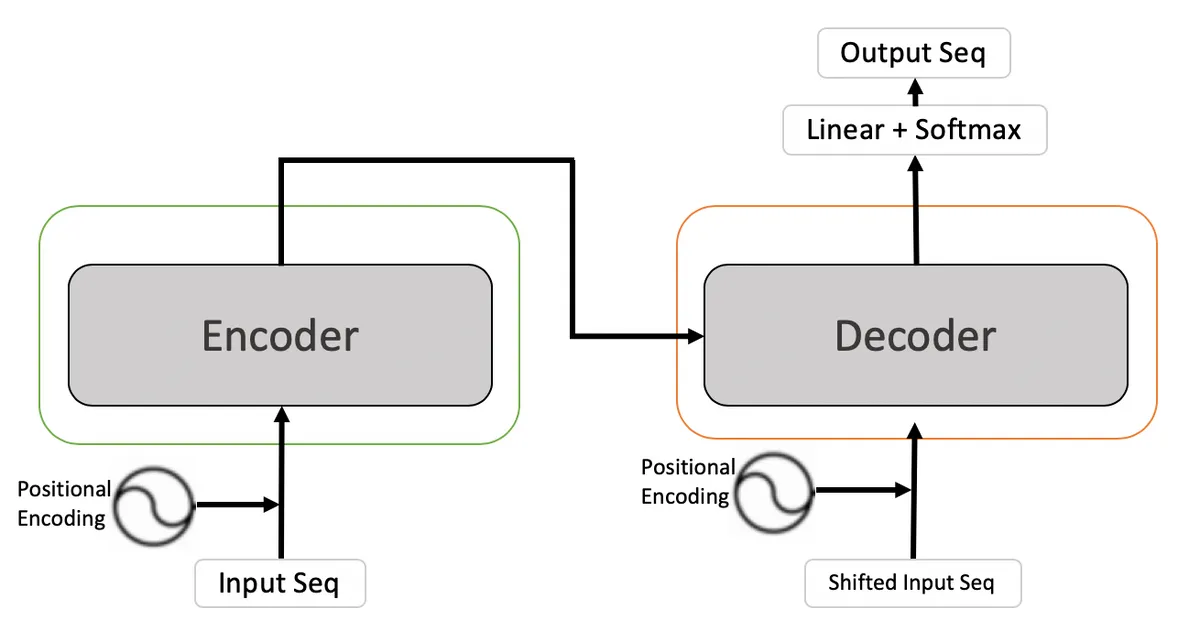
\includegraphics[scale = 0.3]{Images/Tfer.png}
    \caption{High level transformer architecture}
    \label{fig:High level transformer architecture}
\end{figure}

The core mathematical operation in the transformer architecture is the self-attention mechanism, which can be expressed as:
\begin{equation}
    Attention(Q, K, V) = softmax(\frac{QK^T}{\sqrt{d_k}})V
\end{equation}

where Q, K, and V are matrices representing queries, keys, and values, respectively. {$K^T$} represents transpose of Key, {$d_{k}$} is the dimensionality of the key vectors. The attention mechanism calculates a weighted sum of the values based on the similarity between the queries and keys, with the softmax function ensuring that the weights add up to one. This operation can be computed in parallel for all positions in the input sequence, allowing for efficient processing of long sequences.

 \subsection{Attention}
Attention is a mechanism used in neural network architectures that allows the model to selectively focus on different parts of the input data when making predictions. Attention was first introduced in a 2014 paper by Bahdanau et al. for machine translation tasks, and has since been applied to a wide range of natural language processing (NLP) tasks and other domains. The core idea of attention is to compute a set of attention weights that reflect the importance of different parts of the input data for the current prediction. These weights are then used to compute a weighted sum of the input data, which is fed into the rest of the neural network architecture. By focusing on the most relevant parts of the input data for each prediction, attention can improve the performance of neural network models on complex tasks like machine translation and text classification.

Equation: The attention mechanism can be expressed mathematically as:
\begin{equation}
    a_i = softmax(e_i)
\end{equation}
\begin{equation}
    c = sum(a_i * h_i)
\end{equation}

where {$a_i$} is the attention weight for the $i^{th}$ element of the input sequence, {$e_i$} is a score calculated based on the current state of the model and the $i^{th}$ element, {$h_i$} is the hidden state of the {$i^{th}$} element, and c is the context vector, which is a weighted sum of the input sequence. The softmax function is used to ensure that the attention weights add up to one.
 \subsection{Softmax}
Softmax is a mathematical function that is commonly used in machine learning, which takes a vector of real numbers as input and normalizes it into a probability distribution, such that the output values are between 0 and 1 and sum up to 1. The softmax function can be defined mathematically as follows:
\begin{equation}
    softmax(x_i) = exp(x_i) / sum(exp(x_j))
\end{equation}

where {$x_i$} is the {$i^{th}$} element of the input vector x, and the sum is taken over all elements of the vector. The exponentiation and normalization operations ensure that the output values are positive and sum up to 1.
 \subsection{Encoder Architecture}
In the context of neural networks, an encoder is a type of architecture that takes input data and transforms it into a lower-dimensional representation that can be used for downstream tasks like classification, clustering, or generation.

One popular type of encoder architecture is the convolutional neural network (CNN), which typically consists of several convolutional layers followed by pooling layers and a fully connected layer that produces the encoded representation. Another type of encoder architecture is the recurrent neural network (RNN), which processes the input sequence one element at a time, and uses a hidden state to maintain a memory of the previous elements in the sequence. The final hidden state of the RNN can be used as the encoded representation.

A more recent and highly popular encoder architecture is the Transformer, which was introduced in a 2017 paper by Vaswani et al.{\cite{vaswani2017}} The Transformer is a self-attention based neural network architecture that has achieved state-of-the-art results on a wide range of natural language processing tasks. The Transformer encoder consists of several self-attention layers followed by feedforward layers that produce the encoded representation.
.
 \subsection{Decoder Architecture}
The decoder architecture is typically used for tasks such as image or speech generation, language translation, or text generation. It takes the encoded representation produced by the encoder as input and produces an output that is similar to the original input data.

 \subsection{Encoder-Decoder Architecture}
The encoder-decoder architecture is a type of neural network architecture that combines an encoder and a decoder to solve a wide range of tasks. The encoder processes the input data and produces an encoded representation, while the decoder takes the encoded representation as input and generates an output that is similar to the original input data. The encoder and decoder are typically two separate neural networks that are trained jointly using a supervised learning approach. During training, the encoder takes the input data and produces the encoded representation, which is then fed to the decoder to generate the output. The model is optimized to minimize the difference between the output generated by the decoder and the actual output data.

One common type of encoder-decoder architecture is the sequence-to-sequence (seq2seq) model. In a seq2seq model, the encoder processes the input sequence of words and produces an encoded representation, typically in the form of a fixed-length vector. The decoder then takes the encoded representation and generates the output sequence of words in the target language.
\begin{figure}[ht!]
    \centering
    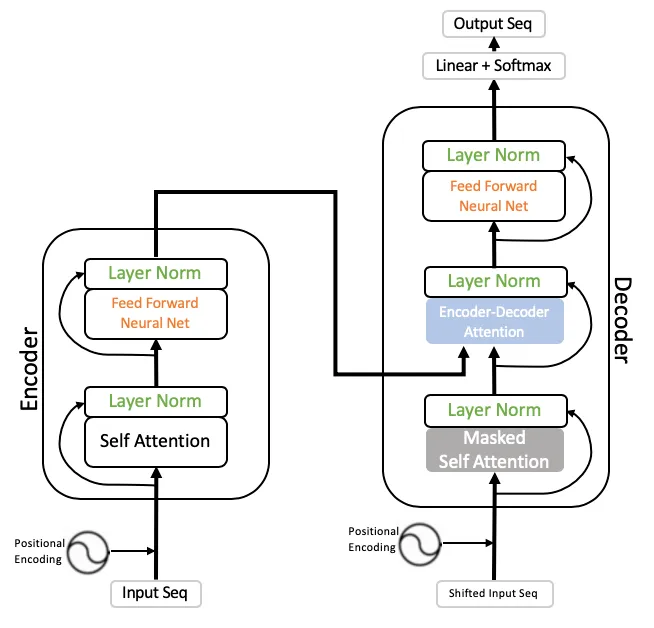
\includegraphics[scale = 0.5]{Images/Encoder_Decoder.png}
    \caption{Encoder Decoder Architecture}
    \label{fig:Encoder Decoder Architecture}
\end{figure}


 \subsection{T5 transformer}
T5\cite{t5} (Text-to-Text Transfer Transformer) is a state-of-the-art transformer-based language model developed by Google. It is based on the same transformer architecture as BERT and GPT-2 but is designed for a specific task of text-to-text transformation. T5 is pre-trained on a large corpus of text and can be fine-tuned on a specific task such as language translation, question answering, or summarization. Unlike other pre-trained language models that are trained for a specific task, T5 is trained to perform a wide range of text-to-text transformations.

T5 uses a variant of the transformer architecture called the Transformer-XL, which is designed to handle longer sequences of text than the original transformer architecture. The Transformer-XL uses a segment-level recurrence mechanism that allows it to handle sequences of arbitrary length, making it well-suited for tasks such as language modeling and text generation.

\begin{figure}
    \centering
    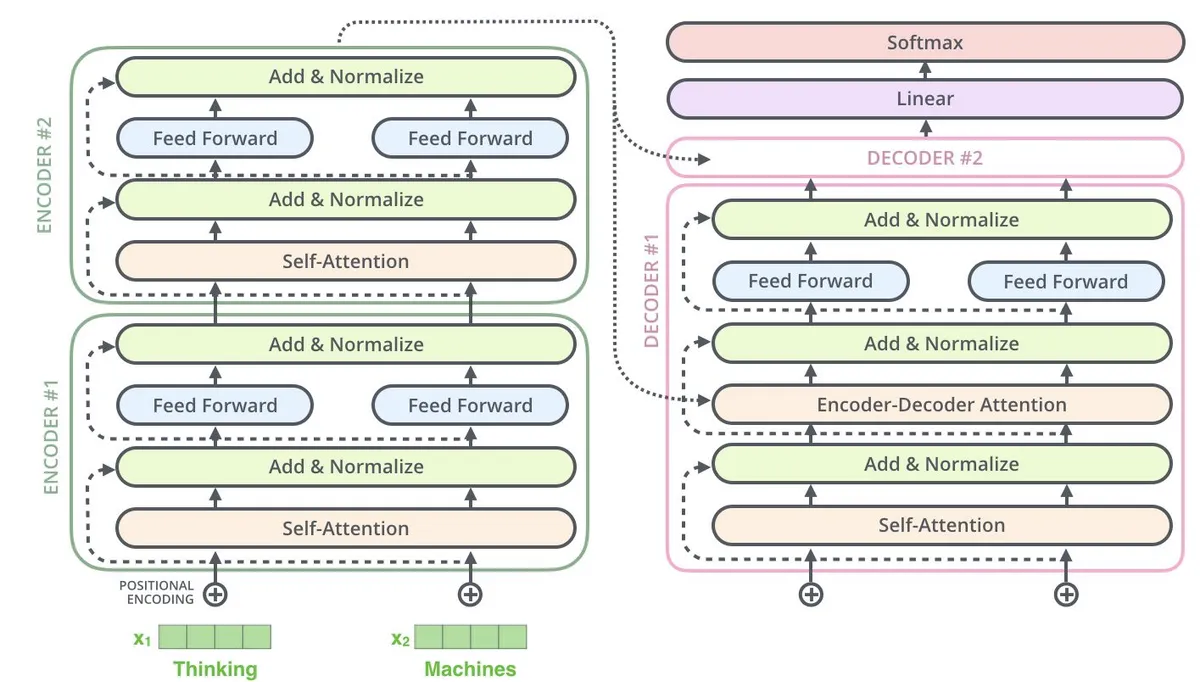
\includegraphics[scale = 0.3]{Images/T5.png}
    \caption{T5 Architecture}
    \label{fig:T5 Architecture}
\end{figure}
T5 has a total of 12 layers, all of which are transformer layers. These transformer layers can be divided into two categories: encoder layers and decoder layers. The encoder layers process the input text, while the decoder layers generate the output text. Within the 12 layers of the T5 model, there are 6 encoder layers and 6 decoder layers.
\begin{enumerate}
    \item {\bfseries Encoder layer}: The encoder layer processes the input text and consists of the following sub-layers:
    \begin{enumerate}
        \item {\bfseries Multi-Head Attention Layer}: It performs attention mechanism on the input sequence to get a weighted representation of each token, taking into account its relationship with other tokens in the sequence.
        \item {\bfseries Feedforward Layer}: It applies a point-wise feedforward network to each position of the sequence independently and identically.
    \end{enumerate}

    \item {\bfseries Decoder layer}: The decoder layer generates the output text and consists of the following sub-layers:
    \begin{enumerate}
        \item {\bfseries Masked Multi-Head Attention Layer}: It performs attention mechanism on the output sequence, but it is masked to ensure that tokens can only attend to previous tokens in the output sequence.
        \item {\bfseries Multi-Head Attention Layer}: It performs attention mechanism on the encoded input sequence, allowing the decoder to focus on relevant parts of the input when generating the output.
        \item {\bfseries Feedforward Layer}: It applies a point-wise feedforward network to each position of the output sequence independently and identically.
    \end{enumerate}
\end{enumerate}
Both the encoder and decoder layers use residual connections and layer normalization to stabilize the training process. The residual connections allow information to pass through the layers easily, while the layer normalization helps in normalizing the inputs to each layer.
\begin{figure}[h!]
    \centering
    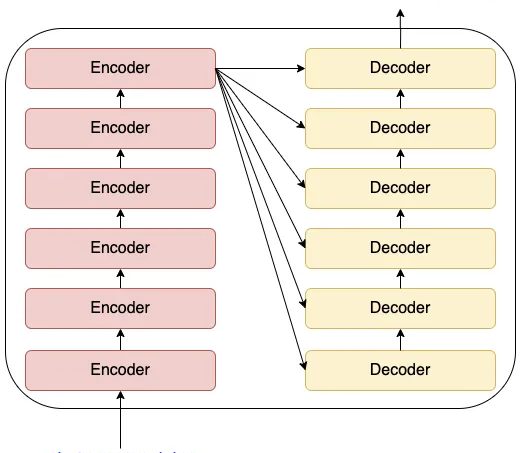
\includegraphics[scale = 0.6]{Images/Tfer_Layers.png}
    \caption{Transformer Layers}
    \label{fig:Transformer Layers}
\end{figure}
\subsection{BLEU Score}
BLEU (Bilingual Evaluation Understudy) score is a metric used for evaluating the quality of machine translation outputs. It measures the similarity between a machine-generated translation and one or more human-generated reference translations. The BLEU score works by comparing the n-gram sequences in the machine-generated translation to those in the reference translations. The BLEU score considers the precision of the n-gram sequences in the machine-generated translation by comparing them with the reference translations. It calculates a modified precision score for each n-gram sequence, which is the number of times the n-gram occurs in the machine-generated translation that also appears in any of the reference translations. This modified precision score is then weighted based on the n-gram length and summed to give a cumulative score. The cumulative score is then normalized by dividing it by the total number of n-grams in the machine-generated translation. The resulting value ranges from 0 to 1, with higher values indicating a better quality translation.
\begin{equation}
    BLEU = BP \cdot \exp\left(\sum_{n=1}^N w_n \log(p_n)\right)
\end{equation}


where:
\begin{itemize}
    \item BP: the brevity penalty term that penalizes generated sentences that are shorter than the reference sentences, calculated as $\min\left(1, \exp\left(1 - \frac{\text{reference length}}{\text{output length}}\right)\right)$
    \item N: the maximum n-gram order to consider
    \item $w_n$: the weight assigned to the n-gram precision, with equal weights typically used (i.e., $w_n = \frac{1}{N}$)
    \item $p_n$: the n-gram precision, calculated as the count of n-grams in the generated sentence that also appear in the reference sentence, divided by the total count of n-grams in the generated sentence
\end{itemize}

The unnormalized BLEU score is a variant of the BLEU score that does not use any length normalization when calculating the score. Unlike the standard BLEU score, which divides the geometric mean of the n-gram precisions by a brevity penalty term, the unnormalized BLEU score simply calculates the geometric mean of the n-gram precisions. While the standard BLEU score is generally preferred due to its ability to handle different-length reference and generated sentences, the unnormalized BLEU score can be useful in certain situations where length normalization may not be necessary or desired, such as when comparing sentence pairs that have the same length.
To calculate the unnormalized BLEU score, the formula is the same as that of the standard BLEU score, except that the brevity penalty term is not used.

\subsection{AdamW}
 The Adam optimizer is widely used in optimizer to adapt the learning rate for each parameter based on the estimate of the first and second moments of the gradients. This makes it possible to use a high learning rate without causing the model to diverge.

However, there is a problem with the Adam optimizer when it comes to weight decay. Weight decay is a regularization technique used in deep learning to prevent overfitting. It works by adding a penalty term to the loss function that encourages the model to have smaller weights. The problem with Adam is that it applies weight decay to all parameters equally, including the ones that shouldn't be regularized, such as the bias terms. This can lead to suboptimal performance.

AdamW is a modification of this Adam optimizer. AdamW solves this problem by decoupling weight decay from the gradient-based optimization step. It achieves this by applying weight decay directly to the weights after each optimization step, rather than including it in the update rule. This means that weight decay is only applied to the parameters that should be regularized, such as the weights, and not to the ones that shouldn't, such as the bias terms. This results in improved performance and better convergence.

\begin{equation}
m_t = \beta_1 m_{t-1} + (1 - \beta_1) g_t \end{equation}

\begin{equation}
v_t = \beta_2 v_{t-1} + (1 - \beta_2) g_t^2 
\end{equation}

\begin{equation}
\theta_t = \theta_{t-1} - \frac{\alpha}{\sqrt{\hat{v}_t} + \epsilon} \hat{m}t - \alpha \lambda \theta{t-1}
\end{equation}

where:\\
$t$ is the current iteration \\
$\alpha$ is the learning rate \\
$\beta_1$ and $\beta_2$ are exponential decay rates for the first and second moments of the gradients, respectively \\
$g_t$ is the gradient at iteration $t$ \\
$m_t$ and $v_t$ are the first and second moment estimates, respectively \\
$\hat{m}_t = \frac{m_t}{1 - \beta_1^t}$ and $\hat{v}_t = \frac{v_t}{1 - \beta_2^t}$ are bias-corrected estimates \\
$\epsilon$ is a small constant to prevent division by zero\\
$\theta_t$ is the model parameter at iteration $t$\\
$\lambda$ is the weight decay coefficient\\

\section{Frontend Theory}
Frontend web development has evolved considerably over the years, with many frameworks and libraries available to help developers create more dynamic and responsive user interfaces. Vue.js and Tailwind CSS are two such technologies that have gained popularity among frontend developers in recent years.

\subsection{Vue.js}
Vue.js is a progressive JavaScript framework that is designed to help developers build scalable and maintainable user interfaces. It is a popular choice for building single-page applications and allows developers to create reusable components that can be easily integrated into their projects. Vue.js also offers a number of powerful features, such as reactive data binding, computed properties, and directives, which make it easier for developers to create dynamic and responsive user interfaces.

\subsection{Tailwind CSS}
Tailwind CSS, on the other hand, is a utility-first CSS framework that allows developers to create custom designs quickly and efficiently. It provides a set of pre-defined utility classes that can be combined to create complex designs without the need for custom CSS. Tailwind CSS also includes a number of features, such as responsive design utilities, hover and focus states, and custom color palettes, that make it easier for developers to create visually appealing designs.

\subsection{Tailwind CSS with Vue.js}
When used together, Vue.js and Tailwind CSS can provide developers with a powerful toolkit for creating modern, responsive web applications. Vue.js can be used to create the core application logic and user interface components, while Tailwind CSS can be used to style and design those components. This allows developers to focus on the functionality of their applications without having to worry about the intricacies of CSS.

One of the key benefits of using Vue.js and Tailwind CSS together is the ability to create modular, reusable components. Vue.js components can be easily styled with Tailwind CSS classes, allowing developers to create custom designs that can be reused throughout their applications. This can save a significant amount of development time and effort, as developers do not have to create custom CSS for each component.

Another benefit of using Vue.js and Tailwind CSS together is the ability to create responsive designs quickly and efficiently. Tailwind CSS includes a number of responsive design utilities, such as breakpoints and screen size classes, that can be used to create designs that adapt to different screen sizes and device types. When combined with Vue.js, developers can create responsive user interfaces that are both functional and visually appealing.

In addition to these benefits, using Vue.js and Tailwind CSS together can also improve the maintainability and scalability of frontend applications. Vue.js allows developers to create clean, organized code that is easy to maintain and update, while Tailwind CSS provides a consistent set of design patterns and styles that can be easily scaled and modified over time.

 \section{Technical Details}
 \subsection{Python}
Python is a high-level, interpreted programming language. It is widely used for various purposes, including web development, data analysis, artificial intelligence, scientific computing, and more. Python is known for its simplicity, ease of use, and readability, making it an ideal language for beginners as well as experienced programmers. Python is generally used in the field of artificial intelligence, with popular machine learning frameworks like TensorFlow and PyTorch built on top of Python. Python's simplicity and ease of use make it an ideal language for prototyping and testing machine learning models.
 \subsection{Numpy}
NumPy is a Python library for numerical computing, specifically designed for working with arrays and matrices. It provides a powerful set of tools for performing mathematical operations on large datasets.
NumPy arrays are stored in memory in a contiguous block, which makes it faster to perform operations on them compared to Python lists. NumPy also provides a set of built-in functions for performing common mathematical operations, such as matrix multiplication, dot products, and trigonometric functions.NumPy also provides functions for indexing and slicing arrays, making it easy to extract specific data from a larger dataset.
 \subsection{Huggingface}
Hugging Face is a company that provides a suite of natural language processing (NLP) tools and libraries, including pre-trained models, datasets, and training pipelines. The company is best known for its work on the Transformers library. The Hugging Face Transformers library provides a wide range of pre-trained models for tasks such as text classification, machine translation, question answering, and more. In addition to pre-trained models, the Transformers library also provides a range of tools for fine-tuning and training models on custom datasets. This includes data preprocessing tools, training pipelines, and evaluation metrics, making it easier for researchers and developers to build and train their own NLP models.
 \subsection{Scipy}
SciPy is a Python library for scientific and technical computing, built on top of the NumPy library. It provides a range of tools for performing scientific computations, including optimization, integration, linear algebra, signal processing, and more. One of the key features of SciPy is its integration with NumPy. SciPy provides a range of functions for performing numerical computations on NumPy arrays, making it easy to perform complex mathematical operations on large datasets.



\chapter{Methodology}
\begin{figure}[ht!]
    \centering
    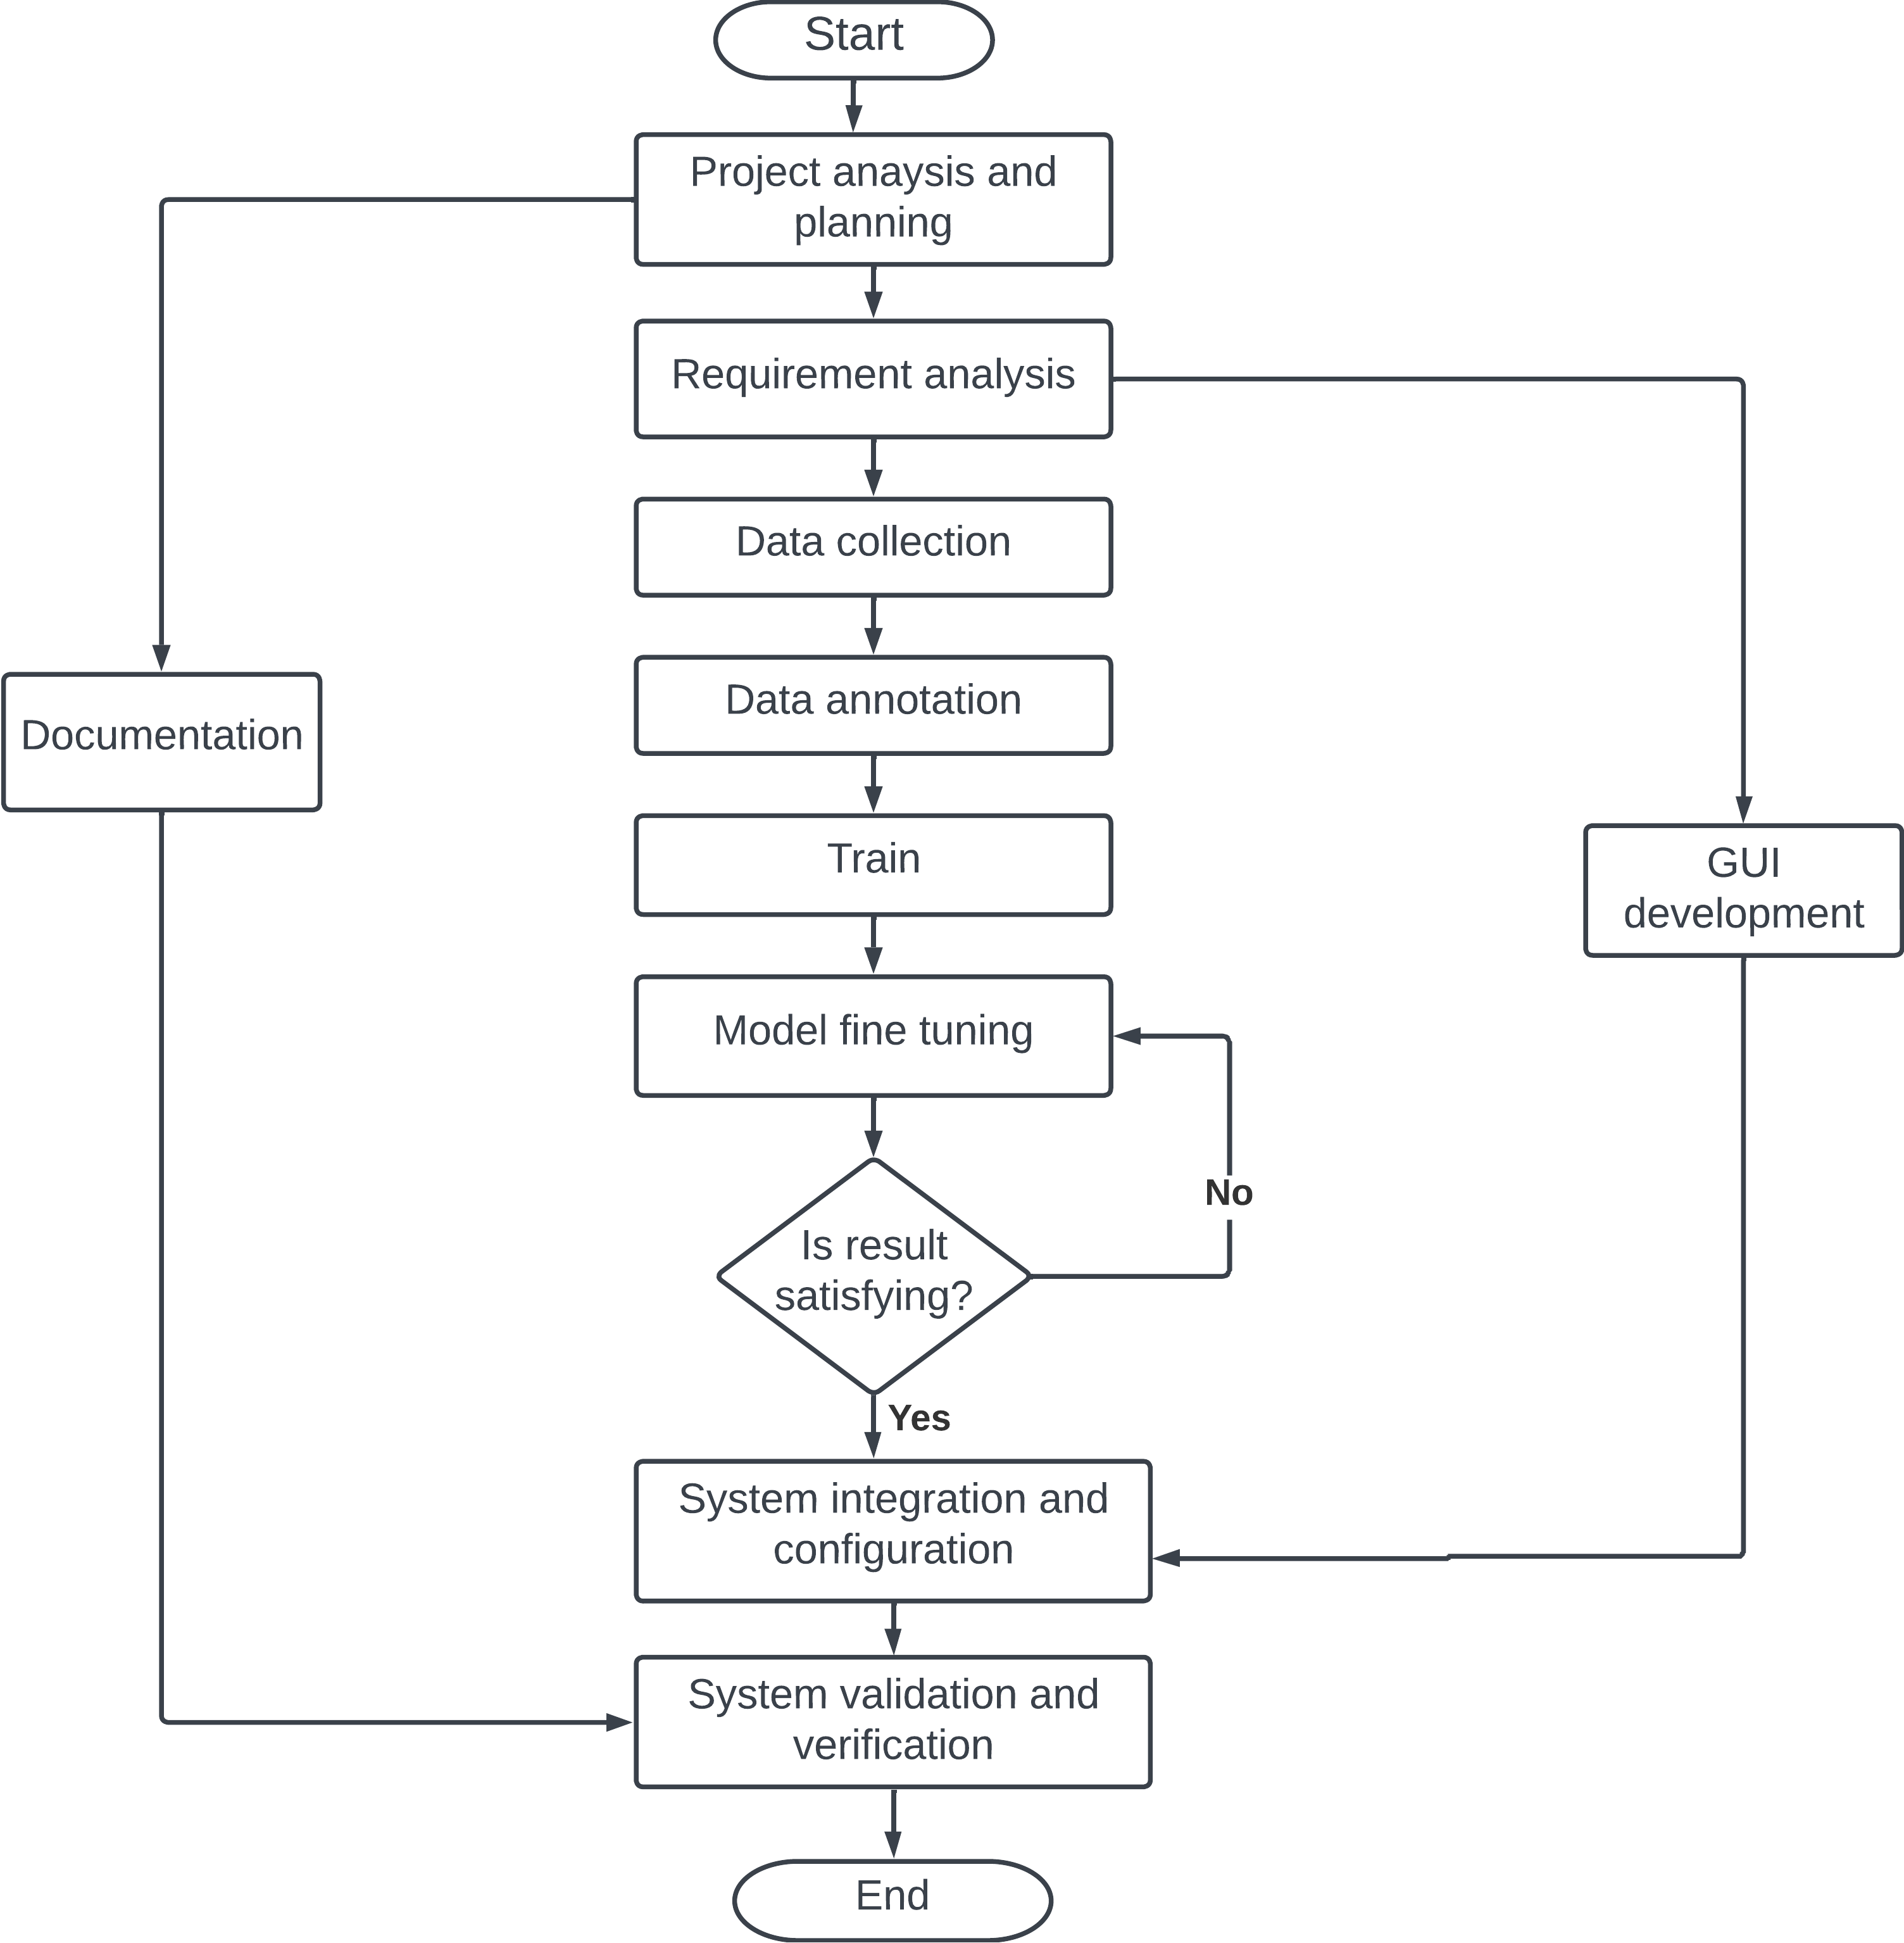
\includegraphics[scale = 0.6]{Images/Methodology.png}
    \caption{Methodology}
\end{figure}
\section{Project Analysis and Planning}
This was the first step of the project. We started analysis of the project. We researched some papers and articles useful for the project which are listed in refrences below. We also make a proper planning and schedule to complete the project. We created a Gantt chart to guide us through the other phases of the project in order to stick with the time available with us to complete the project.

\section{Feasibility Analysis}
The purpose of this feasibility analysis step is to assess the practicality and viability of a T5 transformer model for generating questions from text. The T5 transformer is a state-of-the-art language model that has shown promising results in various natural language processing tasks.  
The T5 transformer model requires significant computational resources to train and fine-tune. The model architecture is complex and requires access to specialized hardware such as GPUs or TPUs. We have assessed the availability of these resources and have found that they are readily available in the market. We used Google Colab as training and fine-tuning platform. Additionally, a large corpus of high-quality text data is required to train and validate the model. We have evaluated the availability and quality of such data and have found that there are various publicly available datasets that can be used for this purpose.

The second half of our project involved generating questions from text based on IoE standards. Unfortunately, there is no readily and publicly available datasets for this task. As part of the feasibility study, we created our own dataset to support our model. While the required data was not readily available, we approached the process of creating the dataset in a professional and systematic manner to ensure that the resulting data was accurate, reliable, and relevant to the project.

To create the dataset, we first defined the data requirements based on the needs of the project. study. This involved identifying the specific data points that were needed to support our analysis, such as customer demographics, purchasing habits, and competitor analysis.
Once the data requirements were defined, we designed the data collection methods to gather the necessary data. This involved developing surveys, conducting interviews, and using other research methods to collect the data. We ensured that the data collection methods were appropriate for the data requirements and that they were designed in a way that would yield accurate and reliable data.
After the data was collected, we organized and analyzed it to create the final dataset. This involved cleaning and formatting the data, identifying outliers or errors, and performing statistical analysis to identify trends and patterns. We ensured that the data analysis was carried out in a rigorous and systematic manner to ensure that the resulting dataset was accurate and reliable.

\section{Requirement Analysis}
Requirement analysis was the second step of the project. It is the process of identifying and documenting the needs and expectations of stakeholders for our software project. Early on, we decided to focius on academic application of this project. Thus our key stakeholders were mainly teachers and students. Next, we gathered, categorized, prioritized and validate requirements. This left us with following requirements :
\begin{itemize}
    \item Generate question from text
    \item Generate question set of selected subjects
    \item Document the project
\end{itemize}

\section{Data collection}
For this project, we collected data from several sources, including the SQuAD dataset, notes, textbooks, and question banks. The Stanford Question Answering Dataset (SQuAD) is a popular benchmark dataset for natural language processing (NLP) research. It consists of a collection of Wikipedia articles and their associated questions and answers, and is widely used for training and evaluating models that perform question answering (QA) tasks. The dataset contains over 100,000 question-answer pairs that cover a broad range of topics, including history, science, literature, and more. Each question-answer pair is associated with a specific paragraph from a Wikipedia article, which provides context for the question and answer. One of the unique features of the SQuAD dataset is that the questions and answers are created by human annotators, rather than generated automatically. This ensures that the dataset contains high-quality, accurate information that is representative of how humans ask and answer questions.

In addition to the SQuAD dataset, we also used textbooks and question banks as a source of additional training data. We selected a set of textbooks that covered following subjects :
\begin{itemize}
    \item Organization and Management
    \item Engineering Professional Practice
    \item Energy, Environment and Society
    \item Software Engineering
    \item Object Oriented Analysis and Design
\end{itemize}
These subjects were chosen as a composition that provides a mix of both computer-based and non-computer based subjects. Also, some of these subjects show the limitations of our model. We used them to extract additional question-answer pairs that were not present in the SQuAD dataset. We also used question banks from various sources to supplement our training data.
To collect the data from the textbooks and question banks, we employed a combination of manual and automated methods. We manually reviewed the textbooks and question banks to identify relevant questions and answers, and then used automated tools to extract the data and format it in a way that could be used for training our model.


\section{Data Annotation}
In order to maintain quality of generated questions,
data annotation is necessary. Annotation involves the process of checking the quality of questions.  First part of our data annotation was to remake our subjectwise data into SQuAD format to ensure consistency in training and fine tuning data. In our project, we utilized manual annotation to annotate the collected data.  Since, SQuAD data was handpicked, we also did the same to keep the quality of questions. The second part of the project required generating questions from subjects in form of IoE based question set. It meant we had to determine the types of questions to be generated from the given text. Just because a question is sound and valid doesn't mean it could be asked in the exams. The annotation process was done by a team of trained annotators who were
provided with clear guidelines and instructions for labeling the data. Ensuring consistency and accuracy in the annotation process was a critical component of this project. To achieve this, we provided our annotators with a detailed set of guidelines and rules for labeling the data. Additionally, we implemented regular quality checks to ensure that the annotation was being done correctly and consistently. This involved reviewing a sample of the annotated data on a regular basis to check for any errors or inconsistencies. If issues were identified,
we would provide additional training to the annotators to ensure that they were following the guidelines correctly.
\section{Data Split}
In this step, the dataset was split into two parts. 90\% of the dataset was used to train the model and the rest 10\% of the data was used to validate the model. AdamW optimizer was used to optimize the model.  
\section{Pretraining and Finetuning}
We used the T5 model for this project because is well-suited for question generation task due to its ability to perform both sequence-to-sequence and text-to-text tasks.
To pretrain a T5 model for question generation, we needed a large corpus of text data that includes both source text and target questions. Thus, we chose SQuAD. SQuAD was chosen ahead of its peers due to the combination of high-quality data, diverse topics, challenging questions, and a standardized evaluation metrics. Datasets like NewsQA don't cover a variety of topics. Similarly, SQuAD v2.0 includes unanswerable questions which aren't being dealt in this project. Similarly, TriviaQA is sourced from quiz bowl competitions, which are known for their difficult and esoteric questions. Thus, TriviaQA may not be representative of the types of questions that people ask in real-world settings.

Once we had SQuAD, you used the T5 model to pretrain on the text-to-text task of generating questions from source text. We used the "text-to-text" version of T5 and trained it on a combination of question-answer pairs and source-answer pairs. 
The training of model had following parameters.
\begin{verbatim}
    dataloader_workers=4
    epochs= 10
    learning_rate = 1e-3
    max_length = 512
    train_batch_size = 4)
    valid_batch_size = 32)
\end{verbatim}
It is important to fine-tune the pre-trained model on the specific downstream task of question generation using supervised learning. Thus, we used a smaller, more targeted dataset for fine-tuning, manually generated from aforementioned subjects, to adapt the pre-trained model to our specific use case.

\section{Evaluation}
To evaluate the quality of the generated questions, we used the Bilingual Evaluation Understudy (BLEU) score, which is a widely used metric for evaluating the similarity between the generated questions and the reference questions. The following BLEU score was obtained by taking arithmetic mean of 10 comparison between generated questions and reference questions for validation set. 
\begin{verbatim}
    BLEU_1 = 54.98
    BLEU_2 = 30.13
    BLEU_3 = 16.56
    BLEU_4 = 7.74
\end{verbatim}
This gives the unified BLEU score 0.208.
This result may look bad at first glance but if we compare it to the best OQPL models, we aren't very far off.
\begin{verbatim}
    BLEU_1 = 55.60
    BLEU_2 = 31.37
    BLEU_3 = 16.79
    BLEU_4 = 8.27
\end{verbatim}
This gives the unified BLEU score 0.219.\cite{lopez2021simplifying}

\section{System Integration and Configuration}
During this step, all the components of the system were integrated to form a single program. The integration testing was also performed to ensure that the system as a whole works fine.

\section{Documentation}
We began documentation of our project at the very start. By documenting the project from start to finish, we ensured that everyone involved in the project understands the goals, requirements, and processes. This documentation will also serve as a reference for future projects, making it easier to build on the success of the current project.
\section{GUI Development}
GUI development was its own project. We took it parallelly along with system. 
\subsection{Requirements Gathering}
The first step in the development process was to gather requirements for the web application. The requirements were defined by us and documented in a requirements document. The document included  design and branding guidelines.
\subsection{Wireframing}

Once the requirements had been defined, a wireframe was created to provide a visual representation of the user interface. The wireframe was created using Figma and included the main components and layouts of the application, such as the , main content areas, and form inputs. The wireframe was reviewed and approved by the team members before proceeding to the next step.

\subsection{Planning the Architecture}
The next step was to plan the architecture of the web application. The architecture was designed to be scalable and maintainable, with reusable components and modules. Vue.js was chosen as the frontend framework, and Tailwind CSS was chosen as the CSS framework. The API was developed using Node.js and Express.js.

\subsection{Developing the Frontend}
The frontend was developed using Vue.js and Tailwind CSS. The components and modules were developed to be reusable, allowing for efficient development and maintenance. Vue.js was used to handle the application's state, and Tailwind CSS was used to style the components and layouts. The frontend was tested extensively to ensure that it met the requirements and was visually appealing.


\subsection{Integration and Testing}
Once the frontend and backend had been developed, they were integrated and tested. The frontend was connected to the API using fetch api, which allowed for easy data fetching and posting. The integration was tested to ensure that the frontend and backend were communicating correctly and that data was being displayed and updated correctly.

\section{Model Architecture}
 To generate questions from text using the T5-base model, the input to the model is a concatenation of the text to generate questions from and a special separator token "<sep>". The T5 model then applies a series of transformer layers to the input to generate a sequence of output tokens, which can include both question words and question marks.

Each transformer layer in the T5-base model consists of three sublayers: multi-head self-attention, a feedforward neural network, and layer normalization. The multi-head self-attention layer allows the model to attend to different parts of the input sequence and capture long-range dependencies. The feedforward neural network applies non-linear transformations to the output of the self-attention layer, while layer normalization ensures that the output of each sublayer has a consistent distribution.

The T5 model is trained using a combination of maximum likelihood estimation and self-supervised learning objectives. During training, the model learns to generate questions from text by predicting the next token in the output sequence given the input sequence and previous tokens. The model is optimized to minimize the negative log-likelihood of the correct output sequence given the input.
So the number of parameters to be learned are: 

The number of parameters in a single transformer layer is:

\begin{equation}
n_{params} = (4 * d_{model}^2 * n_{heads}) + (4 * d_{model} * d_{ff}) + (2 * d_{model})
\end{equation}

where:

$d_{model}$ is the dimensionality of the model's hidden state

$n_{heads}$ is the number of attention heads

$d_{ff}$ is the size of the feedforward neural network

\begin{equation*}
n_{params} = (4 * 768^2 * 12) + (4 * 768 * 3072) + (2 * 768)
\end{equation*}

For T5-base with 12 layers, the total number of learnable parameters is: 
\begin{equation*}
n_{params} = 12 * [(4 * 768^2 * 12) + (4 * 768 * 3072) + (2 * 768)] = 220,027,520
\end{equation*}
.


\chapter{System design}
\section{Overview of System Architecture}
\begin{figure}[ht!]
    \centering
    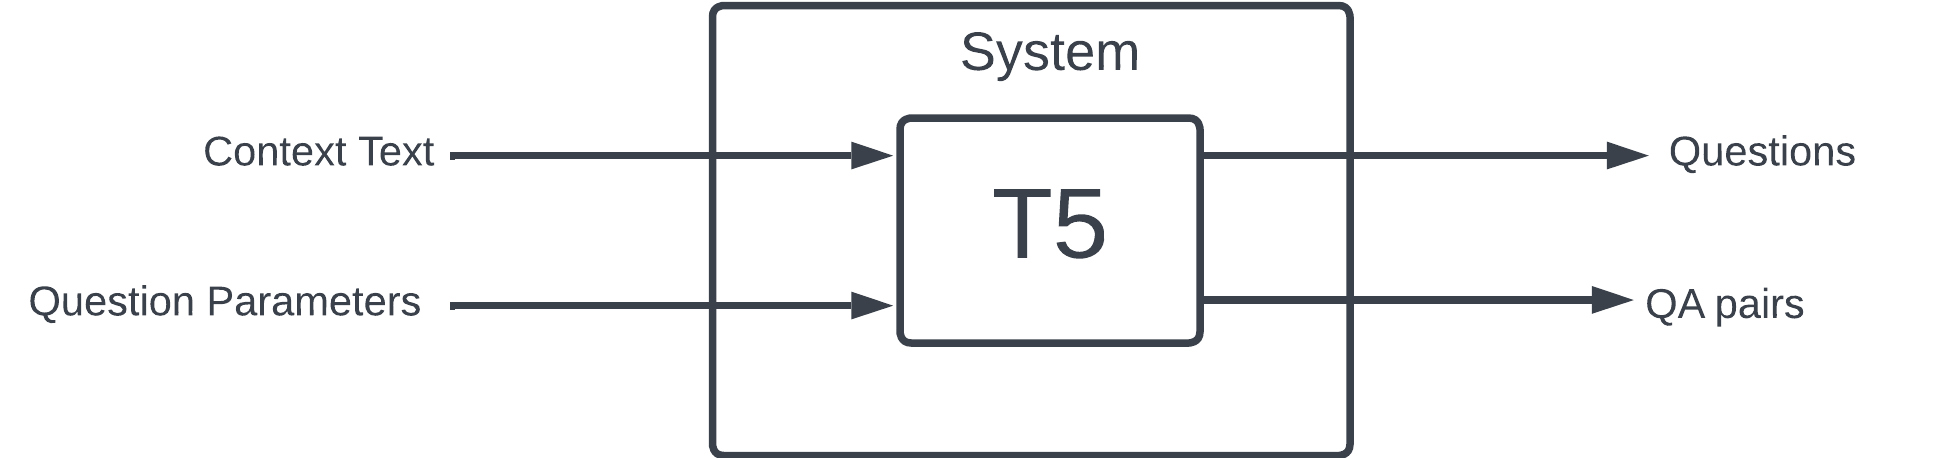
\includegraphics[scale= 1]{Images/Overview.png}
    \caption{Overview of system architecture}
\end{figure}

The user provides context text and question parameters to the system. The system consists of a single T5 model.The model does the pre-processing of inputs. This includes tokenization and encoding of the inputs. The pre-processed input is then used by the T5 model for generating the output questions and/or question-answer pairs. The output generated by the T5 model is then post-processed to format it appropriately.  The final output is returned to the user.
\subsubsection*{Subjectwise Question Generation}
The second part of our model focuses on subject-wise question generation, where users provide subjects and allocate marks to each chapter. Upon receiving the user's input, the system processes the subjects and mark allocations, organizing the information for further analysis. This system also employs a T5 model for generating questions based on the provided subjects and mark distribution. The T5 model is utilized to generate questions aligned with the established  IoE based question pattern for each subject.

The mark distribution guides the T5 model in understanding the importance and weightage assigned to each chapter. This ensures that the generated questions cover the chapters in proportion to their allocated marks. The resulting questions undergo a post-processing step to format and structure them appropriately to fit the desired question pattern.

The final output consists of subject-wise generated questions, ready for use in academic assessments, study aids, or self-evaluation. 
\section{Use Case Diagram}
The use case diagram illustrates the interactions between the user and the system. It outlines the various functionalities available to the user and the corresponding actions performed by the system.
\begin{enumerate}
    \item {Select and Select Marks\\}
    The user the user can select a specific subject. Furthermore, the user has the option to modify the distribution of marks allocated to different chapters within the chosen subject.
    \item{Generate Question Set\\}
    Based on the selected subject and the adjusted mark distribution, the user can request the system to generate a question set. The system employs the trained model to generate questions that adhere to the established question pattern for the given subject by IoE. The resulting question set is tailored to the specified subject and mark distribution.
    
    \item{View Results\\}
    Upon completion of the question generation process, the user can choose to view the results. By selecting the "View Results" option, the user gains access to the generated questions and, if applicable, the corresponding question-answer pairs based on the input text and question parameters.
    \item Change Result\\
    While viewing the results, the user has the option to modify or refine the generated questions. The user can make alterations, such as editing, or deleting questions or modifying the mark assigned.

    \item Final Result\\
    Once the desired changes are made, the user can save the modified question set as the final result. This step ensures that the user has control over the content and structure of the generated questions, allowing for customization and refinement.

    \item View PDF\\
    At last, the user also has the option to view a PDF version of the final result. By selecting the "View PDF" option, the user can access a formatted and printable version of the question set, facilitating easy sharing, distribution, or offline usage.
\end{enumerate}

Alternatively, the use case diagram also highlights an alternative functionality:
\begin{enumerate}
    \item Upload and Customize\\
    Instead of providing subjects, provides a text input to the system, which serves as the contextual information for question generation. The system saves this input for further processing and analysis.
    \item Question Parameters\\
    While the text input is saved, the user enters question parameters, such as the number of questions desired, the type of questions (subjective/objective), and whether to include answer options. These parameters define the characteristics of the questions the user wants to generate.
    \item Generate Questions\\
    After entering the question parameters, the user initiates the question generation process by selecting the "Generate Question" option. The system utilizes the trained model to process the saved text input and the provided question parameters.
\end{enumerate}

Similar to subject-based question generation, this also encompasses the generation of questions from provided text input with question parameters, the ability to view and modify the results, and the option to obtain a PDF version of the final question set.
\begin{figure}[ht!]
    \centering
    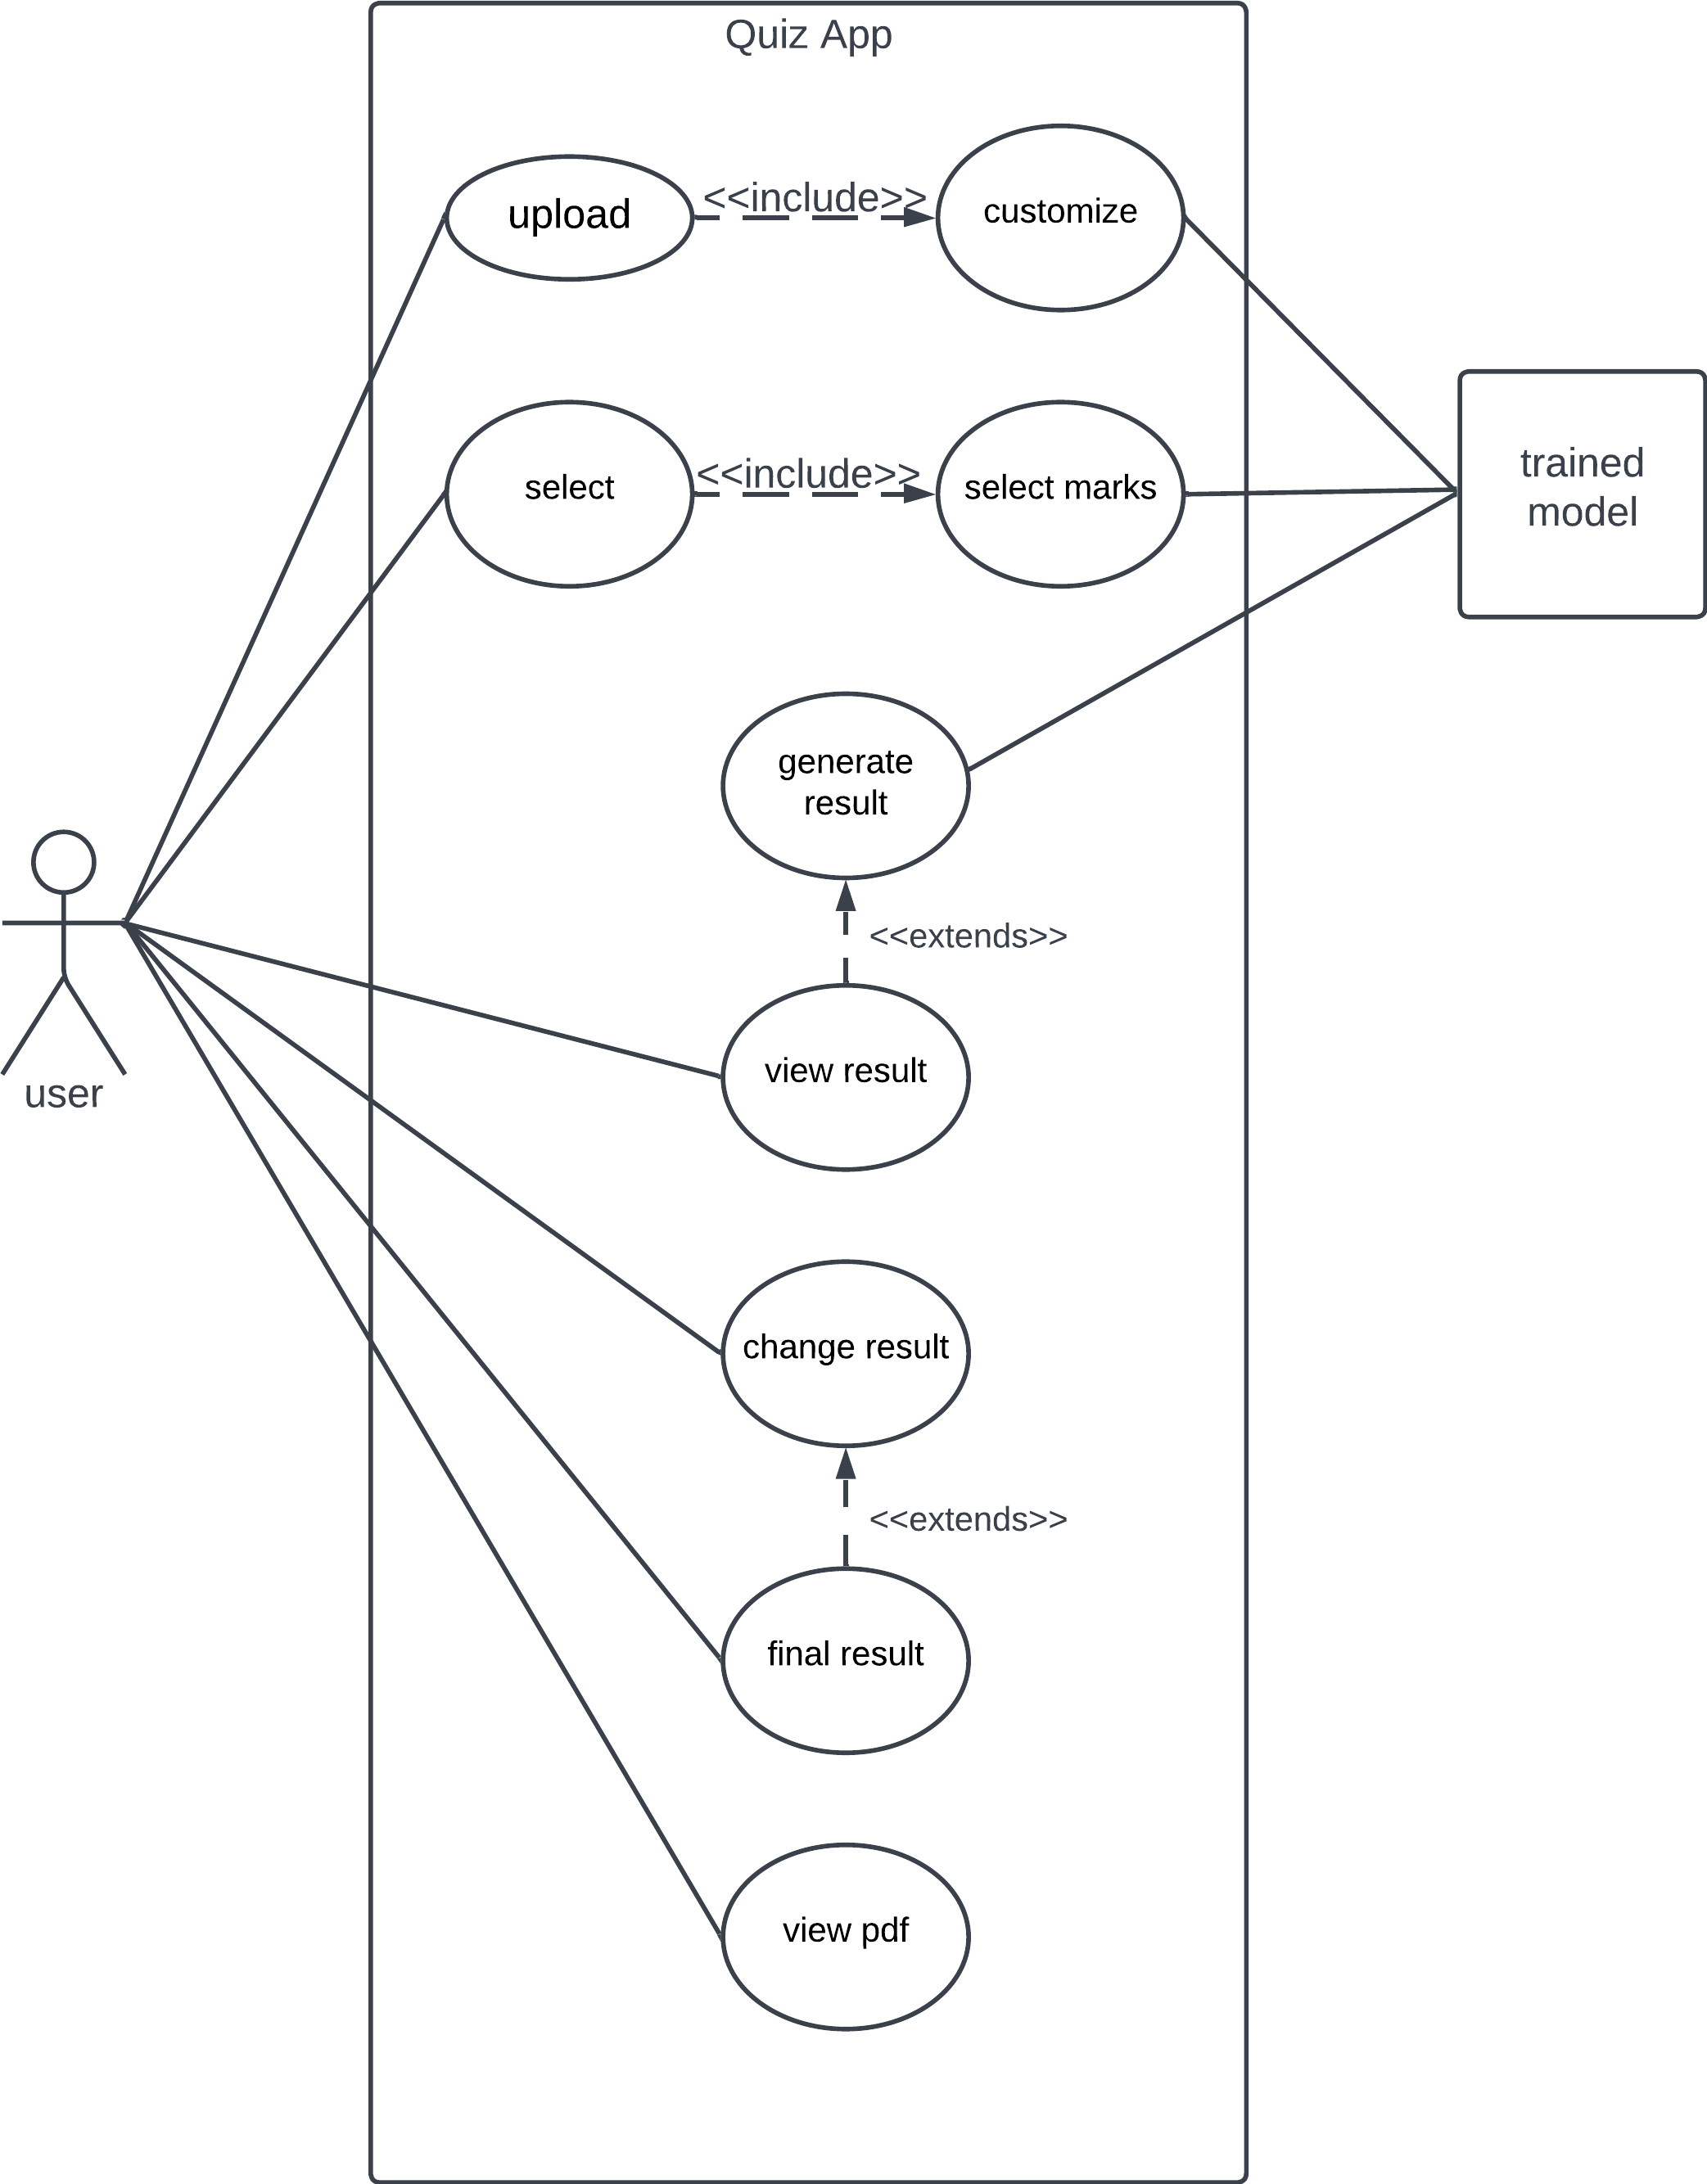
\includegraphics[scale = 0.9]{Images/UCD.png}
    \caption{Use Case Diagram}
\end{figure}
\pagebreak
\section{System Context Diagram}


The system context diagram provides a high-level view of a system and shows its interactions with user(external entity). System represents our system and user is the only external entity that interacts with the system. There are three basic interactions. Use provides context text to the system along with question parameters. The system then returns questions and/or question-answer pairs. This context holds true for generating subjectwise question where the only difference being that the system already has context text and just needs name of subject that points to the text.
\begin{figure}[ht!]
    \centering
    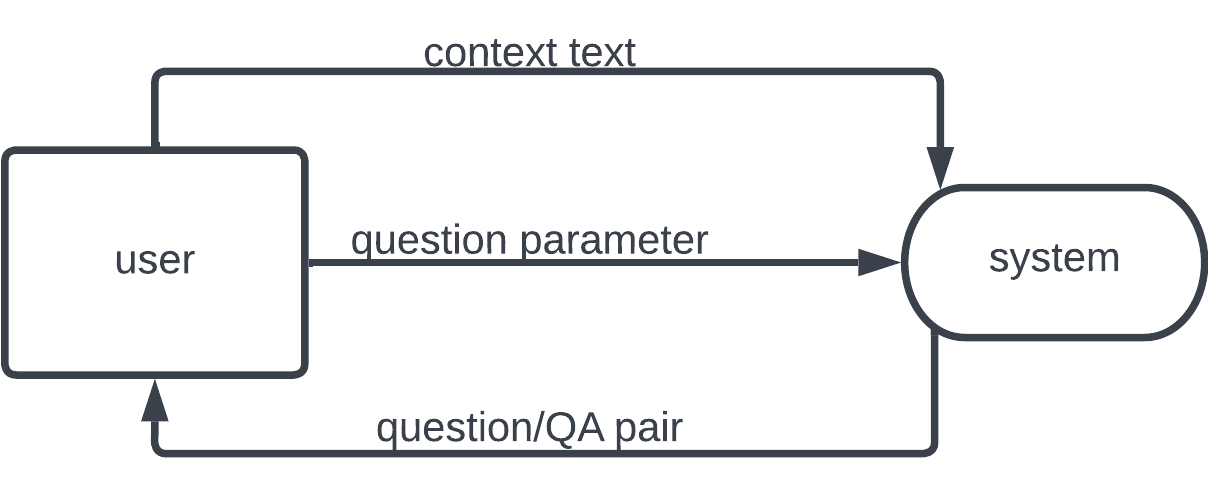
\includegraphics[scale = 1]{Images/Context.png}
    \caption{System Context Diagram}
\end{figure}
\section{Data Flow Diagram}
 The data flow diagram of the system shows the user input as the source of the data flow, with the context text and question parameters flowing into the inference for processing. Similarly, the trained model can also viewed as an input for inference. The system then uses trained model along with text and parameters to provide output. The output of the system would be either questions or question-answer pairs, which would be returned to the user as the final output of the system.
 \\
 Similarly, for the generation of subjectwise questions, the data flow diagram of the system shows the user input as the source of the data flow, with the subject information flowing into the inference for processing. Similarly, the trained model can also viewed as an input for inference. The system then uses trained model along with inputs to provide output. The output of the system would be a questionset, which would be returned to the user as the final output of the system.
\begin{figure}[ht!]
    \centering
    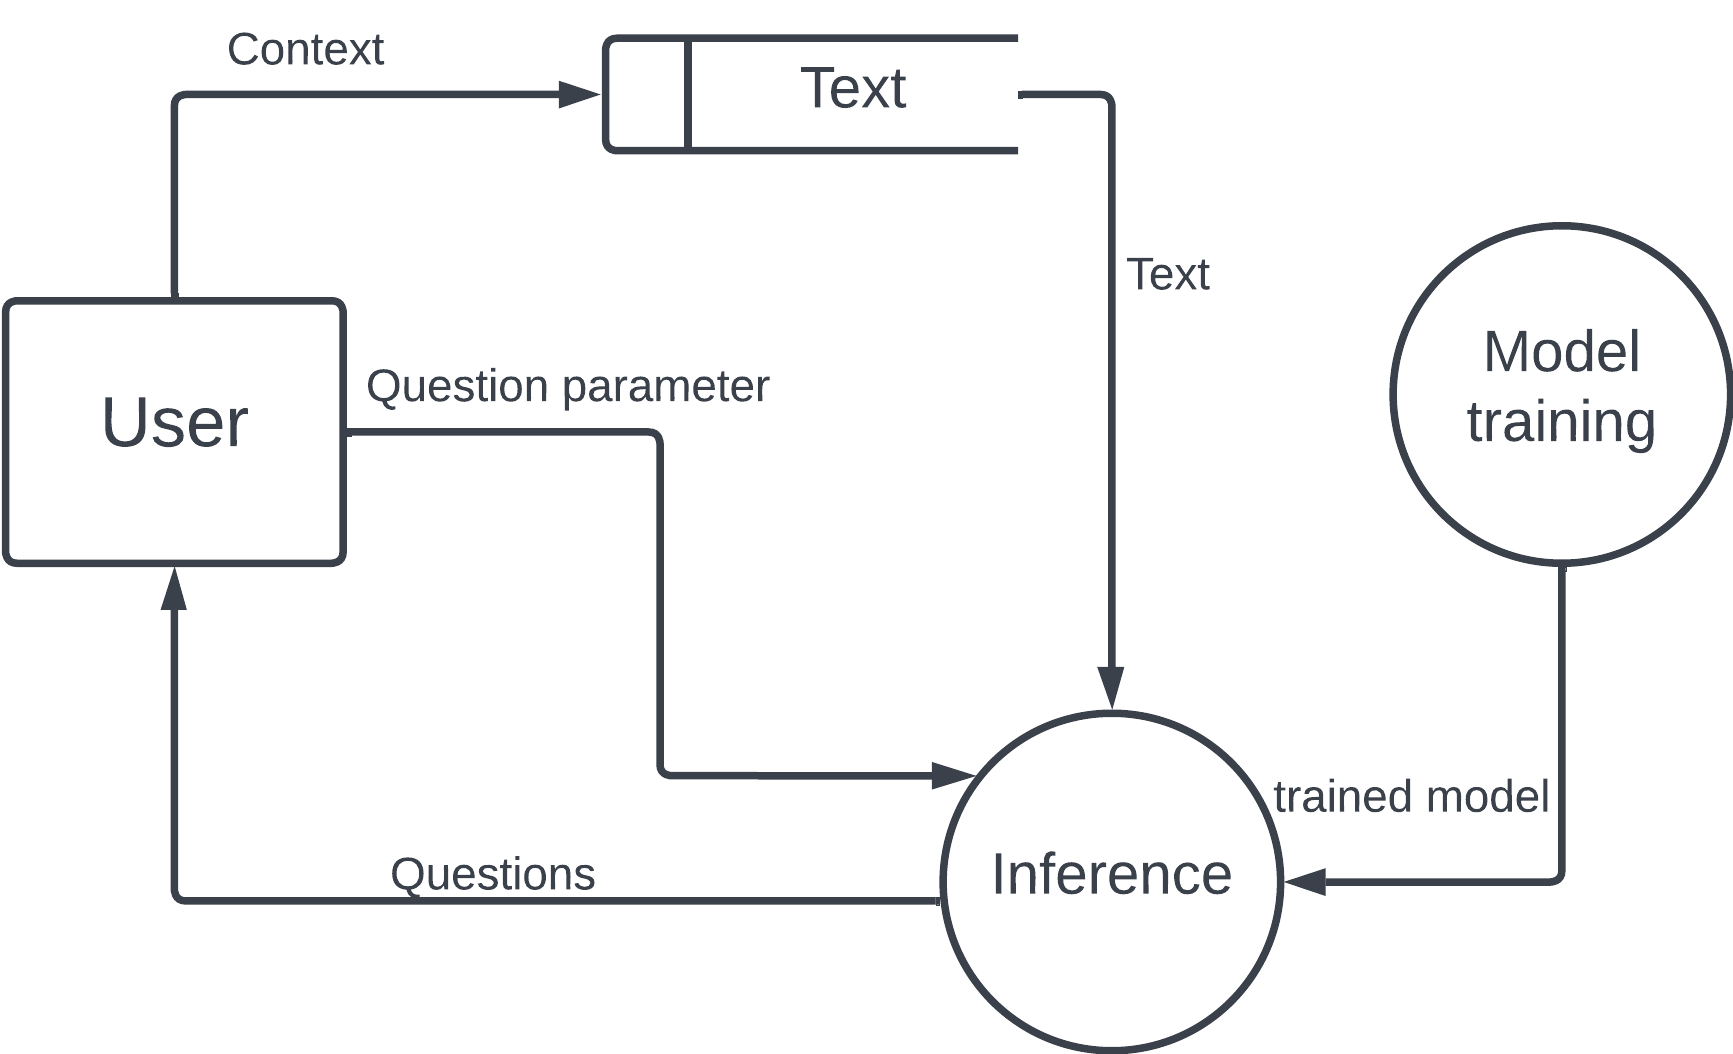
\includegraphics[scale = 0.7]{Images/DFD1.png}
    \caption{DFD for questions from text}
\end{figure}
 
\begin{figure}[ht!]
    \centering
    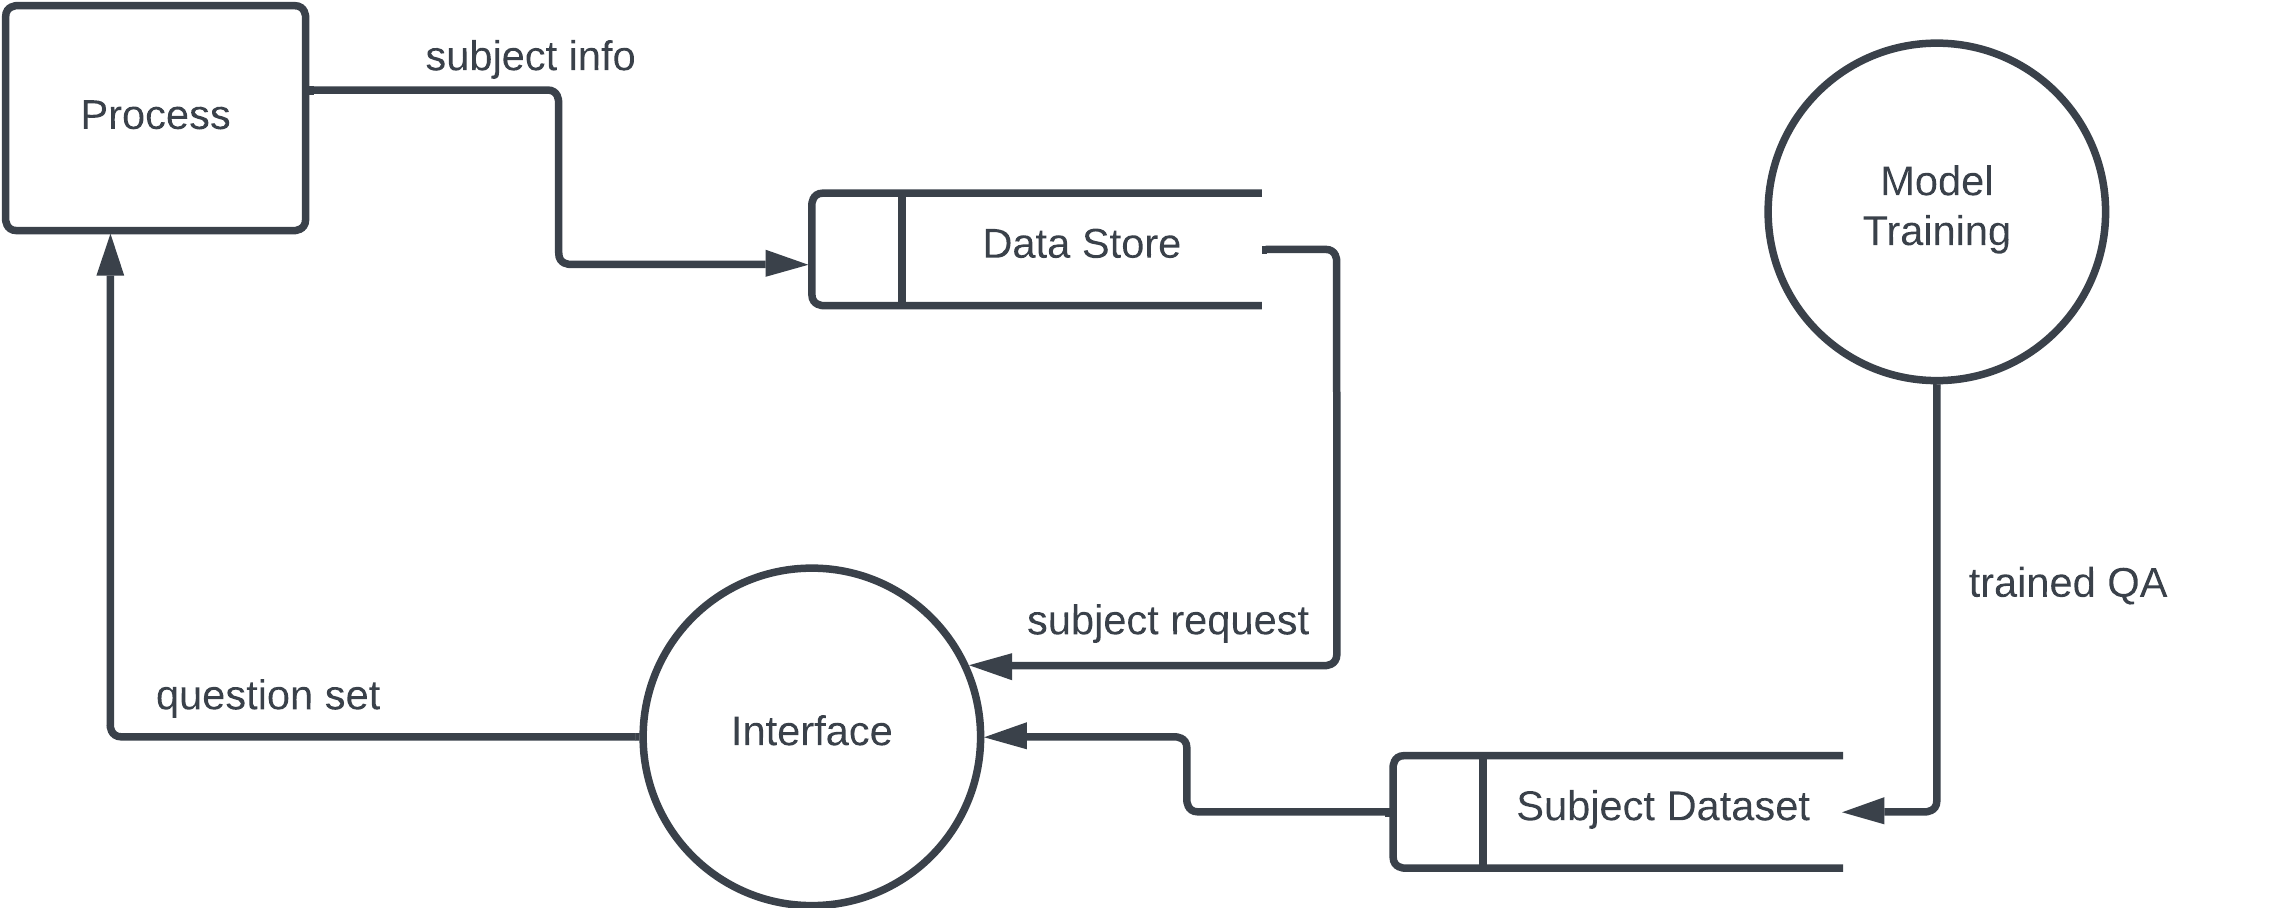
\includegraphics[scale = 0.7]{Images/DFD2.png}
    \caption{DFD for question set from subject}
\end{figure}
\pagebreak
\section{Sequence Diagram}
\begin{figure}[ht!]
    \centering
    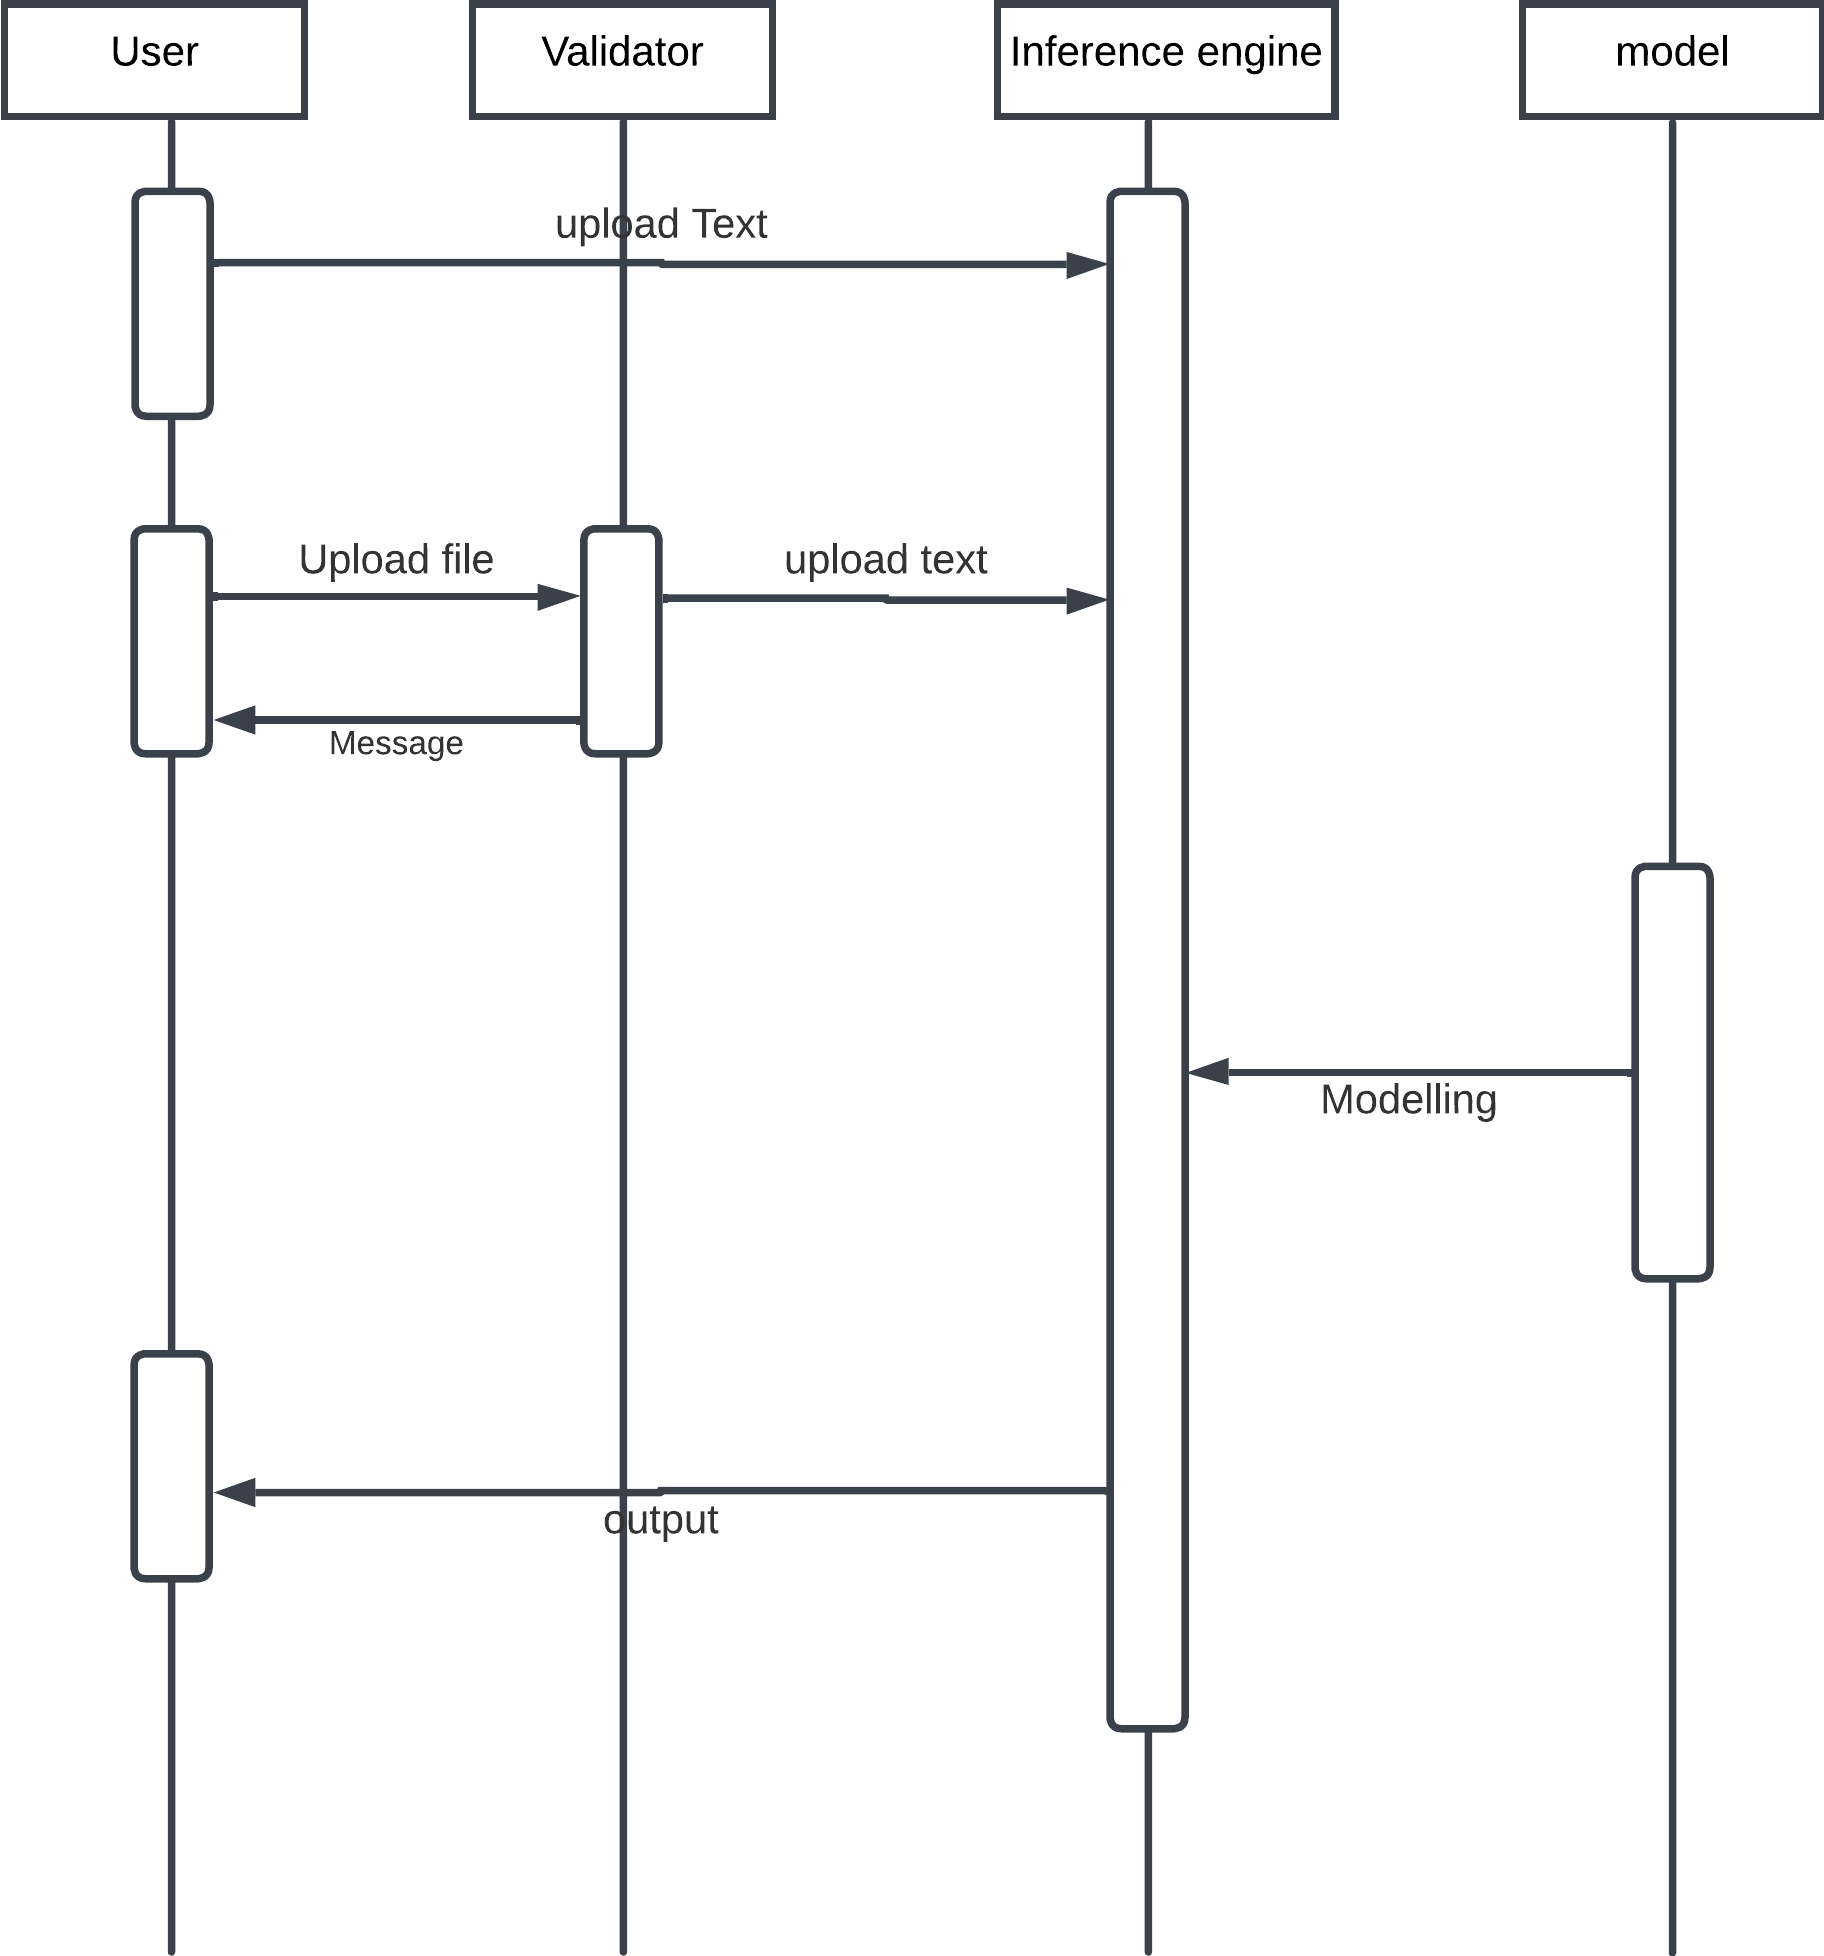
\includegraphics[scale = 1]{Images/SD.png}
    \caption{Sequence Diagram for question from text}
\end{figure}
The diagram depicts the sequence of events in our system. The user inputs text or a textfile. In case of textfile, there is an extra validation step that ensures the text file is acceptable. Next the inference engine gets the input from user and trained model and uses those to infer the output.
\pagebreak
\section{Activity Diagram}
\begin{figure}[ht!]
    \centering
    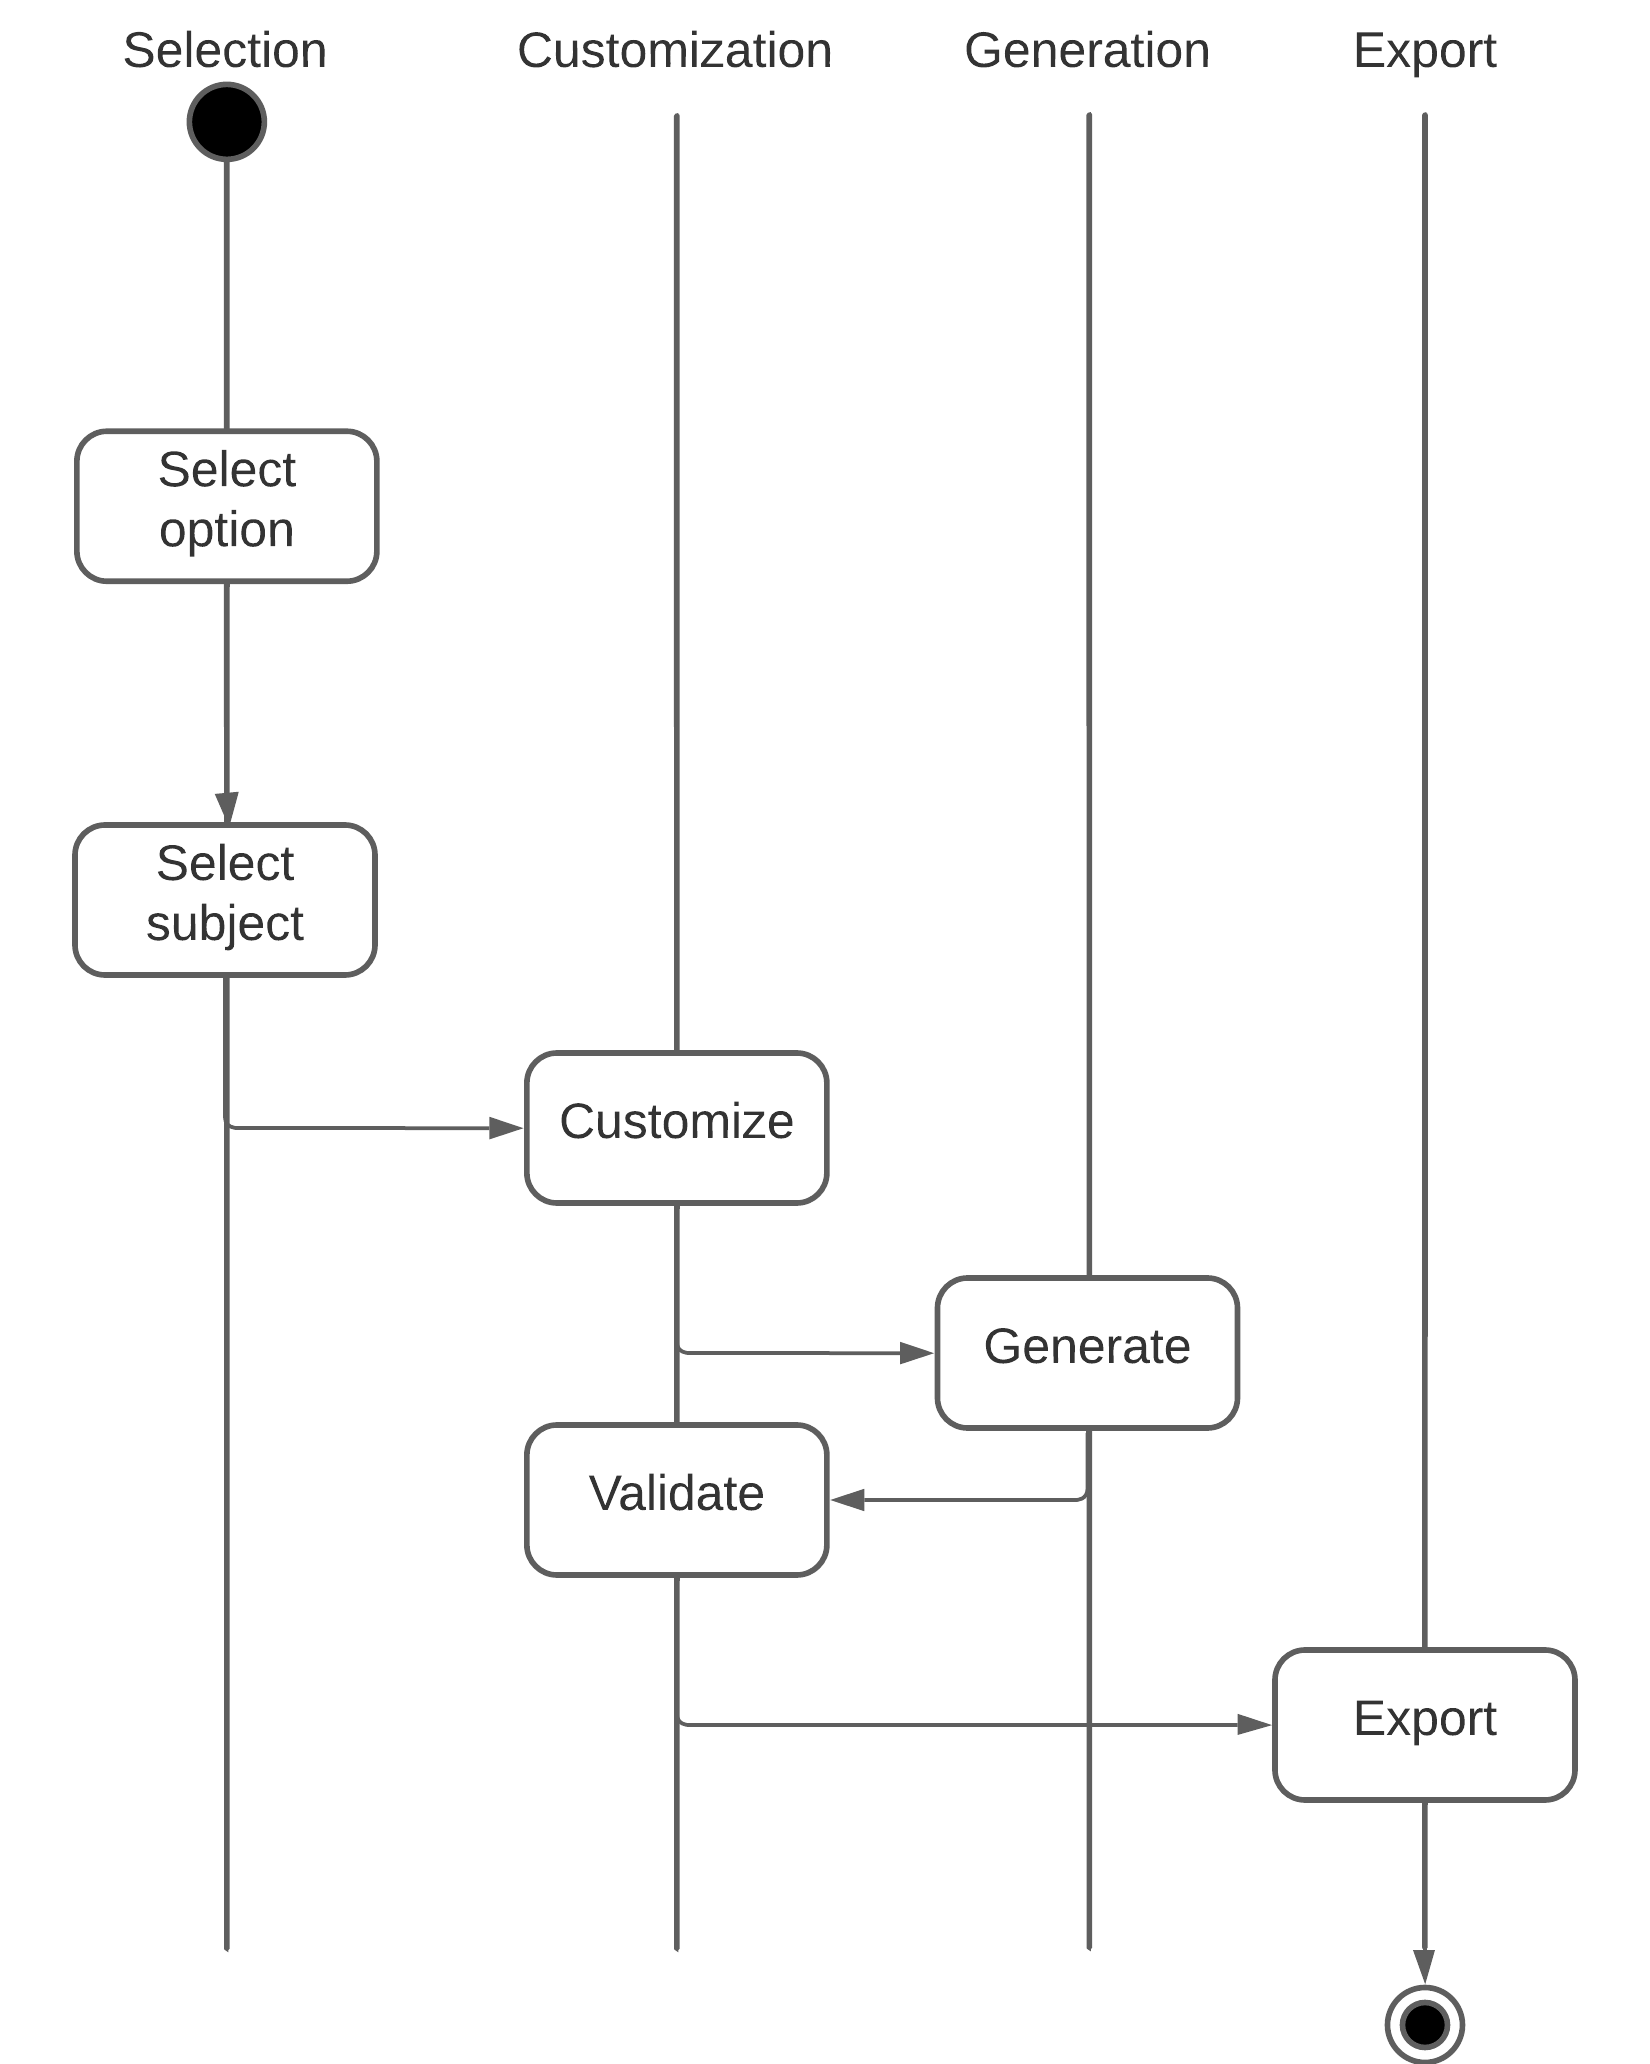
\includegraphics[scale = 1]{Images/Activity.png}
    \caption{Activity Diagram for subjectwise questions}
\end{figure}
The diagram depicts the activities within our system. The user interacts with a select option and selects a subject, User then customizes mark distribution. The system then generates the question set and validates the formatting. Finally, the system can export the text as pdf. 


\chapter{Results \& Discussion}
\section{Model Results}
\begin{tikzpicture}
\begin{axis}[    xlabel={Epoch},    ylabel={Loss},    xmin=1, xmax=10,    ymin=2.5, ymax=4.5,    xtick={1,2,3,4,5,6,7,8,9,10},    ytick={2.5,3,3.5,4,4.5},    legend pos=north east,    ymajorgrids=true,    grid style=dashed,]
 
\addplot[    color=black,    dashed,    ]
    coordinates {
    (1,4.123)(2,3.874)(3,3.671)(4,3.518)(5,3.398)(6,3.299)(7,3.216)(8,3.148)(9,3.092)(10,3.045)
    };
    
\addplot[    color=black,    solid,    ]
    coordinates {
    (1,3.987)(2,3.756)(3,3.589)(4,3.462)(5,3.360)(6,3.277)(7,3.211)(8,3.157)(9,3.114)(10,3.080)
    };
    
\legend{Training Loss, Validation Loss}
 
\end{axis}
\end{tikzpicture}

From the given curve, it can be seen that  the model has reached a saturation point after the 7th epoch. Beyond the 7th epoch, the decrease in the loss is not significant, and the training and validation losses are not improving by a large margin. This suggests that the model has already learned most of the relevant patterns in the data and further training may not improve its performance significantly. Moreover, continuing training for more epochs might lead to overfitting, where the model starts fitting the training data too closely and loses its ability to generalize to new data.

Therefore, it was reasonable to stop training the model at the 10{$^{th}$} epoch, as it has already learned most of the relevant patterns in the data, and continuing training beyond that point did not significantly improve its performance.

\subsection{Question Quality Evaluation}
There is no metric for evaluating the quality of question. Thus, the evaluation were done manually by team members. The model was trained on a particular subject until the question quality was satisfactory,
\subsection{Model Performance Assessment}
There is a distinct lack of metric to assess the performance of a model that generates questions from text. The BLEU score test is the closes metric which still does not provide satisfactory results.
For the following text,
\begin{verbatim}
System design is the process of defining the architecture, components, modules, 
interfaces, and data for a system to satisfy specified requirements
\end{verbatim}
Following questions are possible:
\begin{verbatim}
    "What is system design?"
    "Define system design."
    "What is the definition of system design?
\end{verbatim}
These three questions have the same meaning and are arguably of equal quality. However, the BLEU score of these questions are:
\begin{verbatim}
BLEU score for sentence 1: 0.48
BLEU score for sentence 2: 0.57
BLEU score for sentence 3: 0.37
\end{verbatim}

Thus the system lacks a quality model performance assessment metric.
\subsection{Result Comparison}
\begin{table}[ht!]
    \centering
    \begin{tabular}{c|c|c|c|c|c}
    \hline
{\textbf{BLEU}} &BLEU1 & BLEU2 & BLEU3& BLEU4& unifiedBLEU\\
\hline
    Our Model& 54.98 & 30.13 & 16.56 & 7.74 & 0.208\\
    best OQPL model & 55.60 & 31.37 & 16.79 & 8.27 & 0.219 \\
    \hline
    \end{tabular}
    \caption{Comparison of BLEU scores}
\end{table}
For the best OQPL models, only BLEU scores of 1gram to 4-gram were available.{\cite{lopez2021simplifying}}. We assumed the BP for it to be 1.
\pagebreak
\section{Question Set Evaluation}
 Since there is no automatic evalutaion method for evaluation of question sets, we used Google Forms to collect responses from our classmates regarding the quality of question sets generated by our model. The aim of our evaluation was to assess the model's strengths and areas for improvement.

We designed a survey questionnaire consisting of five evaluation criteria to ensure quality assessment. The participants were asked to rate each criterion on a scale of 1 to 5, where 1 indicated the lowest rating and 5 represented the highest. To collect the responses, we distributed the survey to our classmates using Google Forms. We obtained 14 responses. The obtained responses were analyzed to evaluate the model's performance. 
\begin{enumerate}
    \item {\bfseries Structure}: Ensure the model generates questions as per IoE standards.
    \item {\bfseries Accuracy and Relevance}: Evaluate the accuracy and relevance of the generated questions and corresponding answers with their respective subject.
    \item {\bfseries Language and Grammar}: Assess the model's ability to generate grammatically correct and coherent questions and answers.
    \item {\bfseries Coherence and Cohesiveness}: Analyze the coherence and cohesiveness of the question and answer pairs, ensuring logical flow and proper sequencing.
    \item {\bfseries Consistency}: Evaluate the model's consistency in generating questions and answers across different chapters.
\end{enumerate}

Here are the results for each evaluation criterion:
\begin{enumerate}
    \item {\bfseries Structure}: \\ 
    The average rating for the structure of the generated questions, as per IoE standards, was 4.2 . This indicates questions adhere to IoE standards.
    \item {\bfseries Accuracy and Relevance}:\\ 
    The average rating for the accuracy and relevance of the generated questions and their corresponding answers was [average rating]. This indicates questions and answers were mostly relevant.
    \item {\bfseries Language and Grammar}:\\ 
    The average rating for the model's ability to generate grammatically correct and coherent questions and answers was 4.5. This indicates that the questions and answers are grammatically correct and coherent.
    \item {\bfseries Coherence and Cohesiveness}:\\ 
    The average rating for the coherence and cohesiveness of the question and answer pairs, ensuring logical flow and proper sequencing, was 3.4 . This indicates some inconsistencies in question-answer pairs.
    \item {\bfseries Consistency}:\\ The average rating for the model's consistency in generating questions and answers across different chapters was 4.0 . This indicates that the questions and answers were consistent across chapters.
\end{enumerate}
In tabular form,
\begin{table}[ht]
\centering
\caption{Evaluation Results of Generated Question Sets}
\begin{tabular}{|l|c|p{6cm}|}
\hline
\textbf{Criteria} & \textbf{Average Rating} & \textbf{Evaluation} \\
\hline
Structure & 4.2 & Questions adhere to IoE standards \\
\hline
Accuracy and Relevance & 3.8 & Questions and answers mostly relevant \\
\hline
Language and Grammar & 4.5 & Questions and answers are grammatically correct and coherent \\
\hline
Coherence and Cohesiveness & 3.4 & Some inconsistencies in question-answer pairs \\
\hline
Consistency & 4.0 & Questions and answers consistent across chapters \\
\hline
\end{tabular}
\end{table}


\section{Expert Validation}
In addition to gathering responses from our classmates using Google Forms, we also sought the evaluation of subject teachers to gain further insights into the quality of our AI generated Question Sets. However, the sample size for this aspect of the evaluation was limited, as we only received responses for three out of the five proposed subjects and across ten question sets. Nonetheless, their input provides valuable insights into the quality of the generated questions and helps broaden the perspective beyond student feedback.

While we were able to gather detailed reviews and feedback from our peers, obtaining extensive feedback from teachers proved to be challenging due to various factors, such as time constraints and resource limitations. As a result, their involvement primarily consisted of a thorough study and general feedback rather than an in-depth review. 

The evaluation parameters established for the teachers consisted of four parts: default, partially irrelevant questions, completely irrelevant questions, and out of context. 

The "default" category signifies that the generated questions were meticulously crafted and perfectly aligned with the standards of IoE examinations. These questions not only meet the necessary criteria but also possess the ideal distribution of marks. They represent a  near-perfect fit for the intended purpose.

On the other hand, the "partially irrelevant questions" category represents  a high level of syntactic and semantic accuracy, adhering closely to the requirements of IoE examinations. However, they may fall slightly short in terms of aligning perfectly with the IoE level or allocating appropriate marks. Despite this minor deviation, these questions are still considered remarkable, showcasing a level of quality that is as close to optimal as possible.

Moving forward, the "completely irrelevant questions" category encompasses questions that maintain syntactic correctness but deviate significantly from the semantic requirements of IoE examinations. While these questions may not meet the desired standards, they still be used after adequate refinement.

Lastly, the "out of context" category highlights questions that are unsuitable due to their inadequate quality or lack of relevance to the given syllabus.

To provide a visual representation of the teacher responses, we have prepared pie charts summarizing the evaluation results based on the limited feedback received. The pie chart illustrates the distribution of responses across our four predefined categories: "Default," "Partially Irrelevant Questions," "Completely Irrelevant Questions," and "Out of Context."
\subsection{Visual Representation}
\subsubsection{Engineering Professional Practice}
\begin{figure}[!h]
\centering
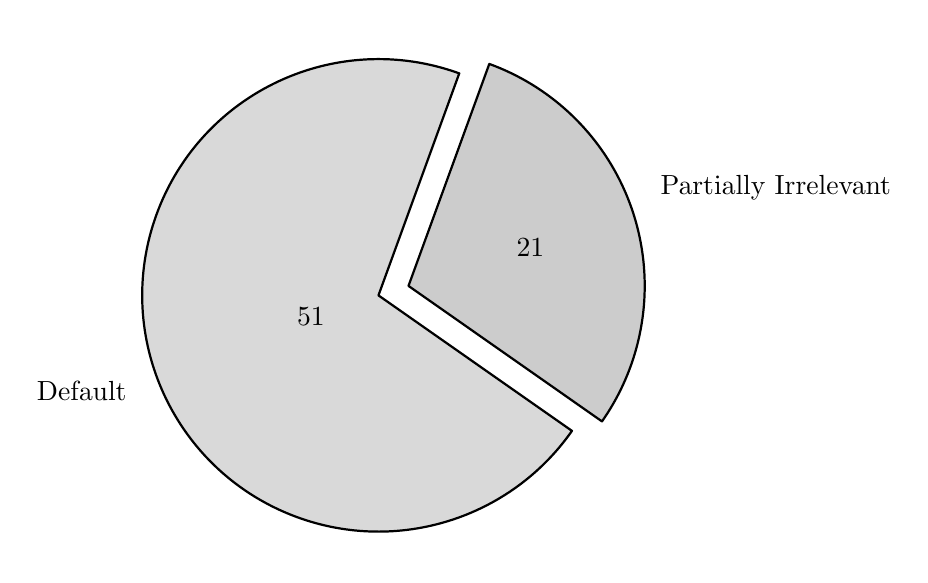
\begin{tikzpicture}
\pie[rotate=70, explode={0.2,0.2}, color={gray!30, gray!40, gray!50, gray!60}, sum = 72]
    {51/Default, 
    21/Partially Irrelevant}
\end{tikzpicture}
\caption{Teacher Responses: Engineering Professional Practice}
\label{fig:pie_chart}
\end{figure}
Figure below presents the evaluation results for Engineering Professional Practice. A total of 10 question sets were evaluated with a total of 72 questions across them. Among the generated questions, 51 were deemed ideal, indicating their alignment with the subject's requirements and IoE standards. These questions required next to no adjustments. The success of the generated questions can be attributed to the nature of Engineering Professional Practice, which is primarily theoretical and does not involve many numerical or open-ended questions. However, 21 questions were categorized as partially irrelevant due to unsatisfactory mark distribution or the presence of repeated questions. This evaluation highlights the effectiveness of the question generation model in producing relevant and suitable questions for this particular subject which doesn't deal with numericals, figures and open ended questions.
\pagebreak


\subsubsection{Object Oriented Analysis and Design}
Figure below illustrates the evaluation outcomes for Object-Oriented Analysis and Design . A total of 20 question sets were evaluated by the teachers with a total of 242 questions across them. The analysis reveals that 79 questions were deemed ideal and aligned with the subject's requirements, signifying their suitability for the IoE examinations without the need for any adjustments.  Additionally, 109 questions were classified as partially irrelevant, indicating that although these questions were grammatically and semantically correct, they fell short of meeting the expected level of the IOE curriculum. The issues identified with these questions primarily revolved around repeat occurrences or necessitated modifications in the allocation of marks. Furthermore, 36 questions were considered completely irrelevant due to their failure to meet the semantic requirements of the subject. Additionally, 18 questions were labeled as out of context, indicating their poor quality or lack of relevance to the syllabus. This evaluation highlights the limitations of the question generation model in producing relevant and suitable questions for this particular subject which deals heavily with figures and open ended questions.  As a text-based model, it faced challenges in generating questions that effectively encompassed the use of figures and successfully addressed the open-ended nature of certain question types. 
\begin{figure}[!h]
\centering
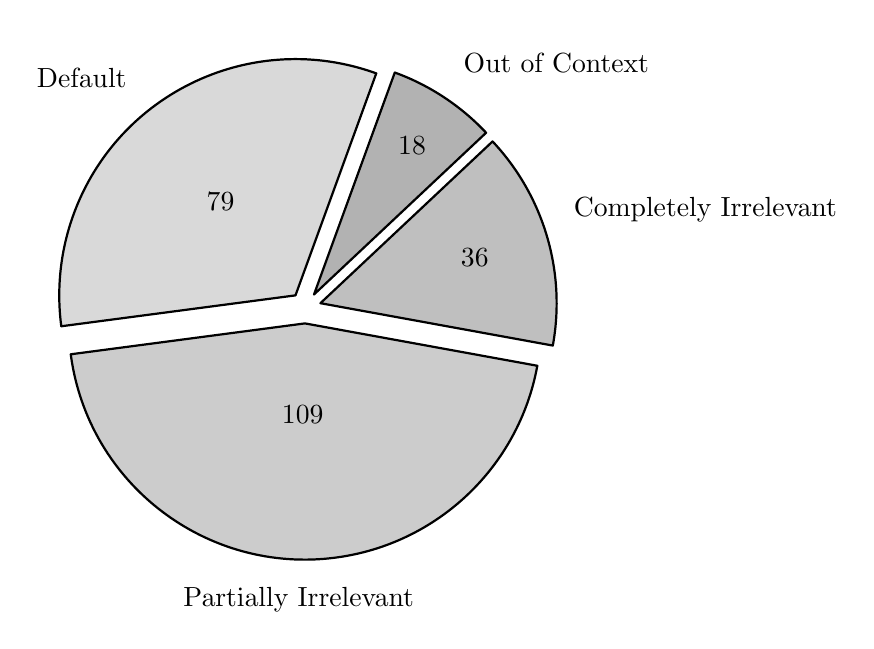
\begin{tikzpicture}
\pie[rotate=70, explode={0.2,0.2,0.2,0.2}, color={gray!30, gray!40, gray!50, gray!60}, sum = 242]
    {79/Default, 
    109/Partially Irrelevant, 
    36/Completely Irrelevant, 
    18/Out of Context}
\end{tikzpicture}
\caption{Teacher Responses: Object Oriented Analysis and Design}
\label{fig:pie_chart}
\end{figure}
\pagebreak

\subsubsection{Software Engineering}
Figure below illustrates the evaluation outcomes for Software Engineering. A total of 149 questions were evaluated across 10 question sets. Out of these questions, 57 were categorized as default, indicating their strong alignment with the subject's requirements and suitability for IoE examinations without any adjustments. However, 54 questions were classified as partially irrelevant, suggesting that they did not fully meet the expected level of the IOE curriculum. These questions either had repeated content or required modifications in mark allocation. Additionally, 21 questions were considered completely irrelevant as they failed to meet the semantic requirements of the subject. Furthermore, 17 questions were labeled as out of context, indicating their lack of quality and relevance to the syllabus. This evaluation underscores the limitations of the question generation model in incorporating figures and addressing the open-ended nature of certain question types, which are prominent aspects of Software Engineering. The majority of Software Engineering deals with processes and charts which is not fully supported by text-based models. Thus,  as a text-based model, it struggled to generate questions that effectively captured these elements, resulting in the higher number of irrelevant and out-of-context questions
\begin{figure}[!h]
\centering
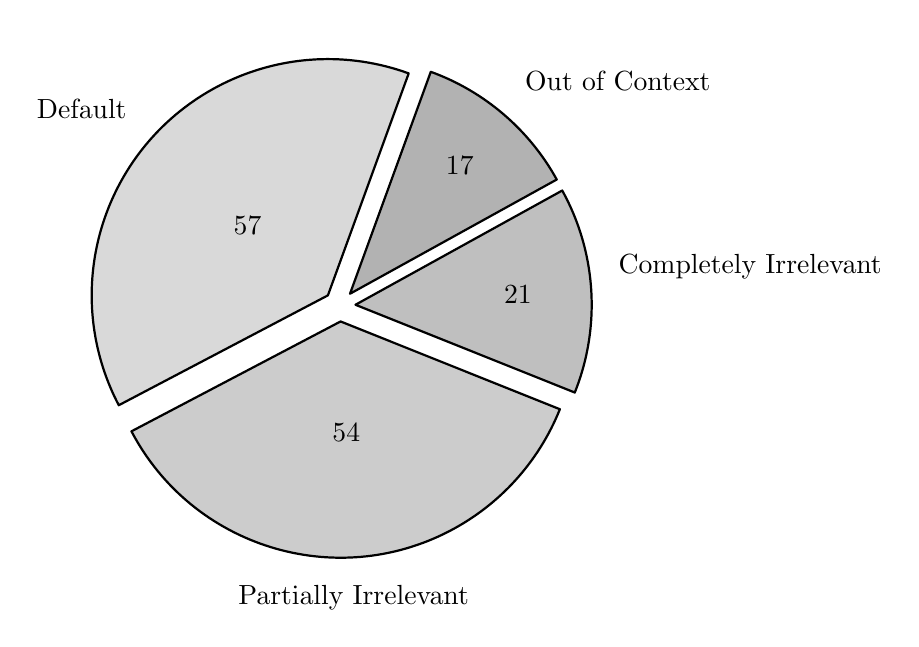
\begin{tikzpicture}
\pie[rotate=70, explode={0.2,0.2,0.2,0.2}, color={gray!30, gray!40, gray!50, gray!60}, sum = 149]
    {57/Default, 
    54/Partially Irrelevant, 
    21/Completely Irrelevant, 
    17/Out of Context}
\end{tikzpicture}
\caption{Teacher Responses: Software Engineering}
\label{fig:pie_chart}
\end{figure}
\pagebreak

In order to gain a comprehensive understanding of the evaluation results across multiple subjects, we have combined the pie charts representing the feedback received for each subject. The following combined pie chart presents an overview of the evaluation outcomes for the three subjects: "Object Oriented Analysis and Design", "Software Engineering", and "Engineering Professional Practice".
\begin{figure}[!h]
\centering
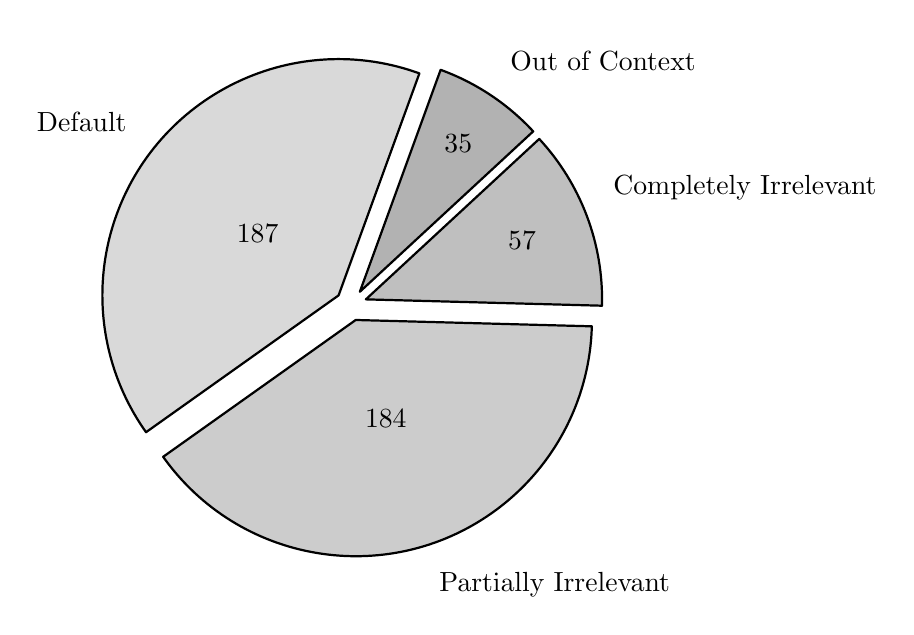
\begin{tikzpicture}
\pie[rotate=70, explode={0.2,0.2,0.2,0.2}, color={gray!30, gray!40, gray!50, gray!60}, sum = 463]
{187/Default,
184/Partially Irrelevant,
57/Completely Irrelevant,
35/Out of Context}
\end{tikzpicture}
\caption{Combined Teacher Responses}
\label{fig:pie_chart}
\end{figure}
\pagebreak

As depicted in the chart, the majority of the responses fell within the "Default" category, indicating that the generated questions were deemed appropriate for IoE examinations and had the correct weightage assigned to them. Almost similar portion of the responses were categorized as "Partially Irrelevant Questions," highlighting instances where the questions were almost in the IoE level, just lacked appropriate marks allocation. Furthermore, a minority of the responses fell under the categories of "Completely Irrelevant Questions" and "Out of Context," signifying instances where the questions did not quite meet the requirements of IoE examinations or were deemed unsuitable due to poor quality or lack of relevance to the given syllabus.




\chapter{Conclusions}
This project on question generation from text using T5 model is a promising application of natural language processing techniques. By leveraging the power of the T5 model, the project was successful to generate high-quality questions from input text. Although the project focused on academic applications of automatic question generation, further extension to this project  can be useful for a variety of applications, such as content creation, and information retrieval.

Throughout the project, several challenges and limitations were encountered. The biggest limitation being length limitations. The T5 model is limited in the length of input that it can take at a time(512 words) and lack of parallel processing options meant that it was difficult to generate questions for long input texts. This also meant that the time to train the model significantly increased. Since training a T5 model is computationally expensive and time-consuming, it limited our ability to experiment with different training data other than SQuAD such as TrivialQA, NewsQA, SQuADv2 and so on. This means that, our claim of SQuAD being the best data set was a result of our preliminary study and not a verified result.  Also, the lack of reliable automatic evaluation tools meant  human evaluation was required, which was expensive and time-consuming.

In conclusion, this project highlights the potential of using state-of-the-art language models like T5 for generating questions and opens up several avenues for future research. This also provides a gateway for furthur academic research such as exploring the use of multimodal inputs such that figures and numerical data are handled as input.  With further advancements in natural language processing techniques, question generation can become an even more valuable tool for various applications in the future.
\chapter{Limitations and Future enhancement}
One limitation of our question generation project, or any question generation project in general using T5 base or any other natural language processing model is that it is not be able to generate questions that are outside the scope of the training data. This means that if the training data is limited to a specific domain or topic, the generated questions may not be as diverse or useful for other domains or topics. For example, we can only generate quality questions for a handful of subjects although we can generate quality questions in a variety of fields.

Another limitation of our project is the semantic relationship between questions and answers. Since it is trained on a question-answer data set, the quality of questions are good. However, the answers (mostly, when they need to be summarized) do not necessarily match the questions semantically. Also, since the model isn't trained for summarization, the answers may not necessarily make sense.   

Future work for a question generation project using T5 base could increasing the number of subjects the model can generate question sets. By extension, this model can also be trained to generate sample mock question set for Engineering License examination. Another area of research could be to develop more advanced evaluation metrics to measure the quality of generated questions. This could involve using human evaluation or other metrics beyond the traditional BLEU score, such as the relevance and coherence of the generated questions. 
% \section{Limitations}
% The project doesn't extend to : 
% \begin{itemize}
%     \item Languages other than English language, Nepali and other languages aren’t supported.
%     \item Implied answers, only explicit answer and key phrases are supported.
%     \item Numericals and figure based questions, only text based questions are supported.
%     \item Apaptive question generation. 
% \end{itemize}
\addcontentsline{toc}{section}{References}
\renewcommand{\bibname}{References}
\bibliographystyle{unsrt}
\bibliography{ref}
\chapter{Appendices}
\addcontentsline{toc}{section}{Appendices}
\section{Sample SQuAD dataset}
{\bfseries Context:}
The War of the Spanish Succession (1701–1714) was a European conflict over who would succeed Charles II as King of Spain. The war involved nearly all of the major powers of Europe, with two main alliances opposing each other: the Grand Alliance, led by Austria, Britain, and the Dutch Republic; and the Bourbon Alliance, led by France, Spain, and Bavaria. It was marked by a series of military engagements, mostly in Italy, the Low Countries, and Germany, where armies were raised, financed and led by a complex and intricate network of coalition governments and the financing systems that supported them.\\
{\bfseries Question:}
What were the two main alliances in the War of the Spanish Succession?\\
{\bfseries Answer:}
The two main alliances in the War of the Spanish Succession were the Grand Alliance, led by Austria, Britain, and the Dutch Republic, and the Bourbon Alliance, led by France, Spain, and Bavaria.
\section{Sample Output}
% The user is greeted with a hamepage that allows the user to either generate questions based on specific subjects for IoE or provide text to generate general text-based questions.
\begin{figure}[ht!]
    \centering
    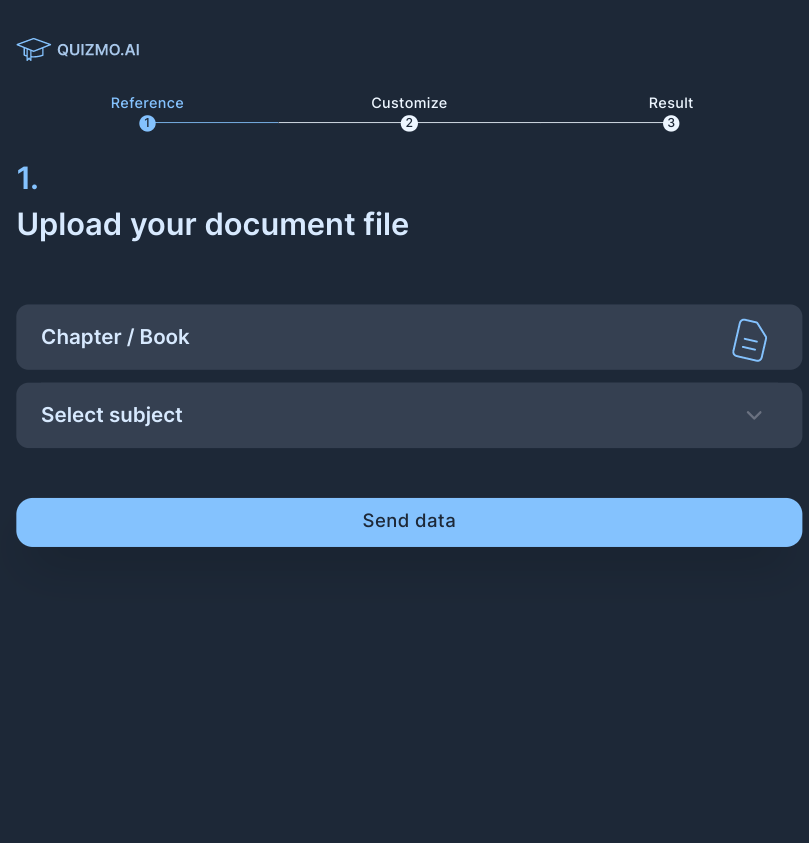
\includegraphics[scale = 0.3]{Images/Page1.png}
    \captionsetup{justification=centering} 
    \caption{Output: HomePage \\ Choose between IoE based question generation and general text-based question generation}
\end{figure}
\begin{figure}[ht!]
    \centering
    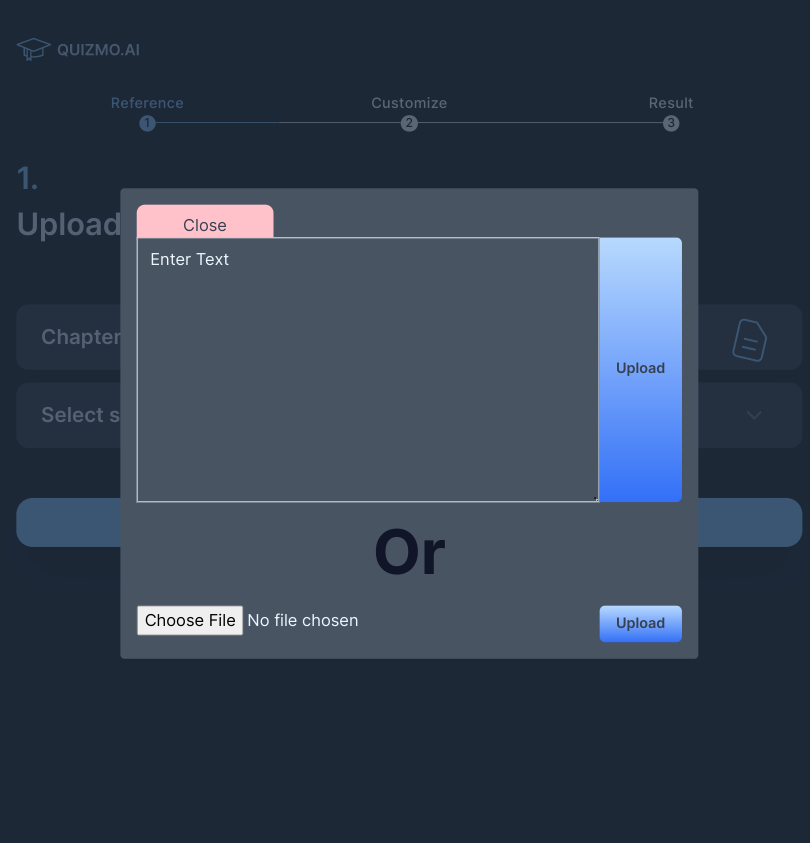
\includegraphics[scale = 0.4]{Images/TextSelect.png}
    \captionsetup{justification=centering} 
    \caption{Output: Text Selection\\ In case of general text-based question generation, either enter text or upload a text file}
\end{figure}
\pagebreak
\begin{figure}[ht!]
    \centering
    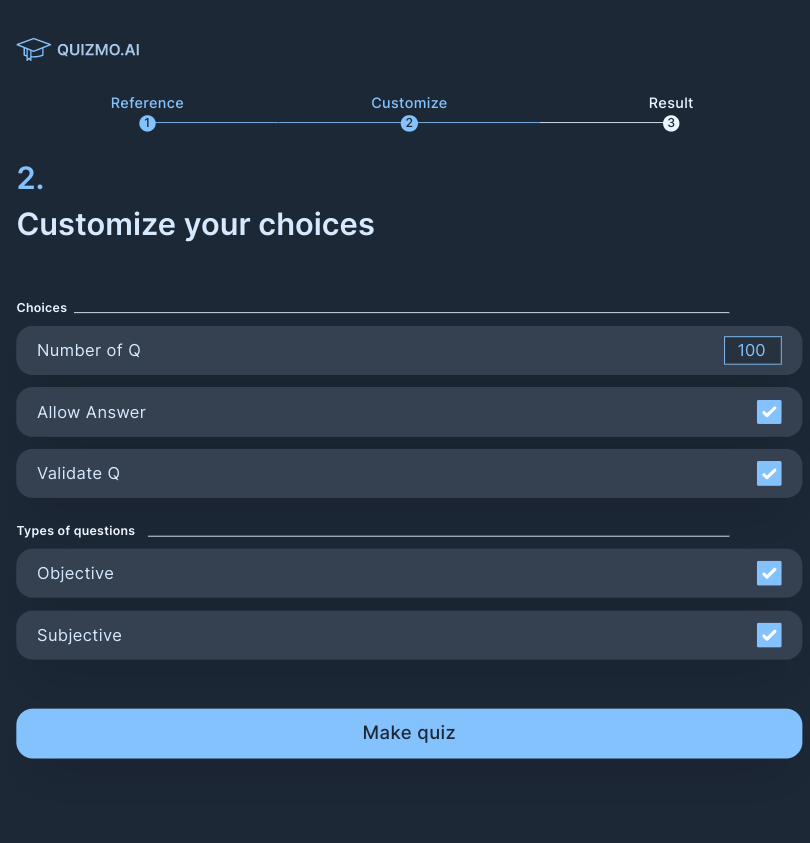
\includegraphics[scale = 0.4]{Images/QuestionCustomization.png}
    \captionsetup{justification=centering} 
    \caption{Output: Question Customization \\ In case of general text-based question generation, choose question parameters like Number of questions, Subjective/Objective questions, Number of questions, etc.}
\end{figure}

\begin{figure}[ht!]
    \centering
    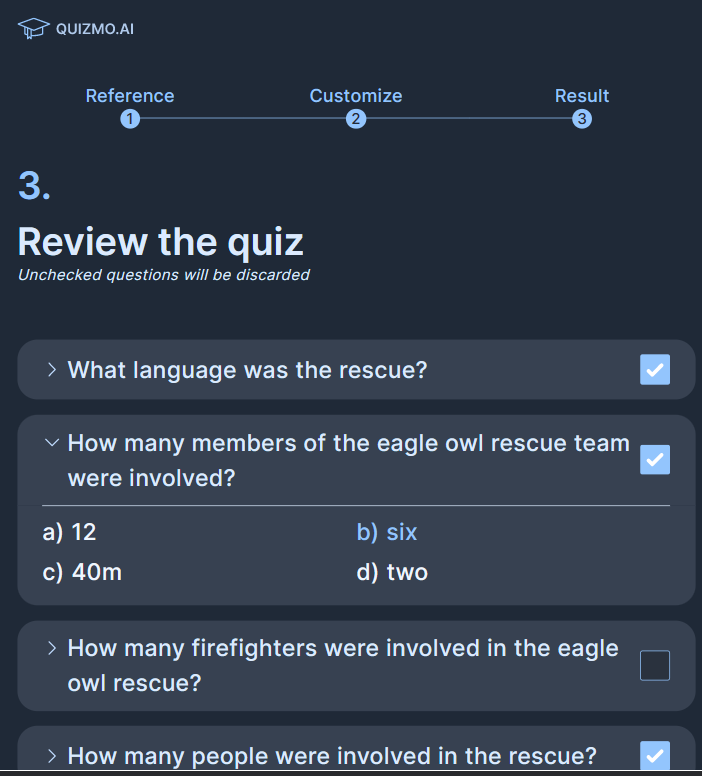
\includegraphics[scale = 0.4]{Images/review.png}
    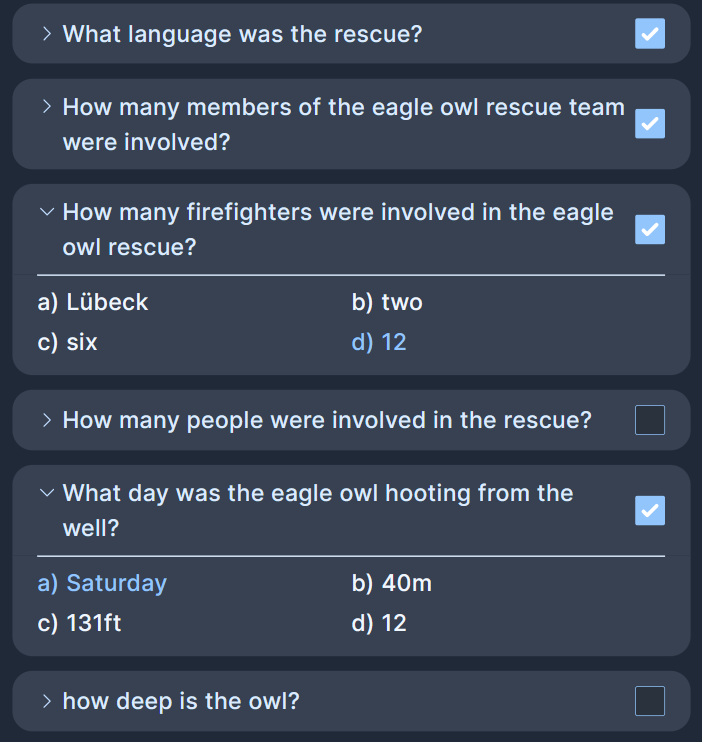
\includegraphics[scale = 0.42]{Images/review2.png}
    \captionsetup{justification=centering} 
    \caption{Output: Question Review \\ Finally review the questions to choose whether to keep or discard them.}
\end{figure}
\pagebreak
\begin{figure}[ht!]
    \centering
    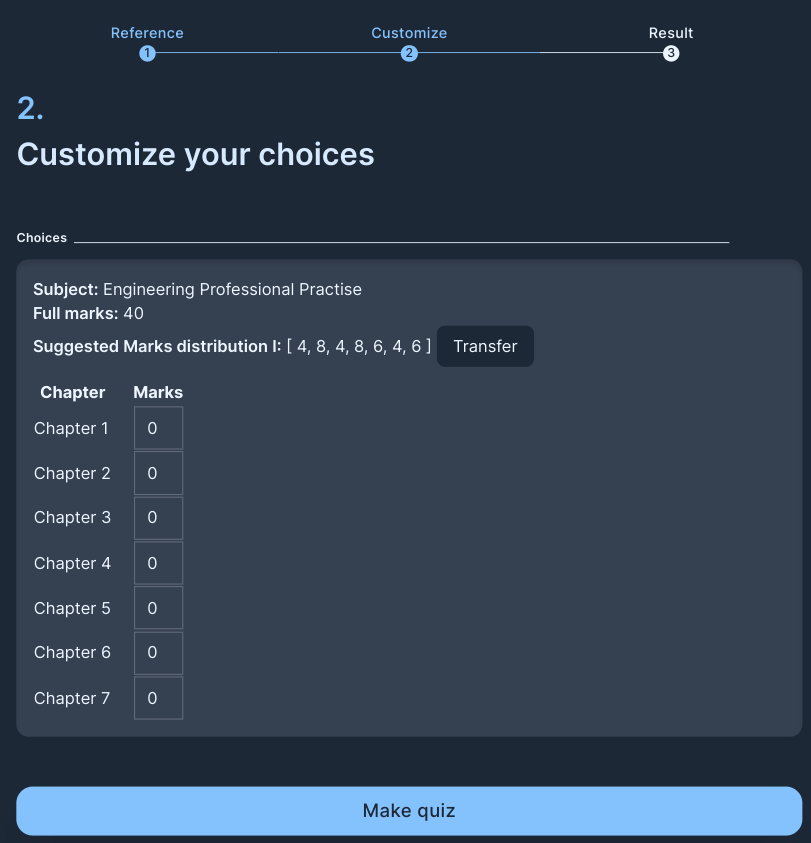
\includegraphics[scale = 0.4]{Images/MarkDistributionforSubjectwise.png}
    \captionsetup{justification=centering} 
    \caption{Result: Mark Distribution customization \\ In case of IoE-based question generation, choose mark distribution instead of question customization parameters.}
\end{figure}
\pagebreak
\begin{figure}[ht!]
    \centering
    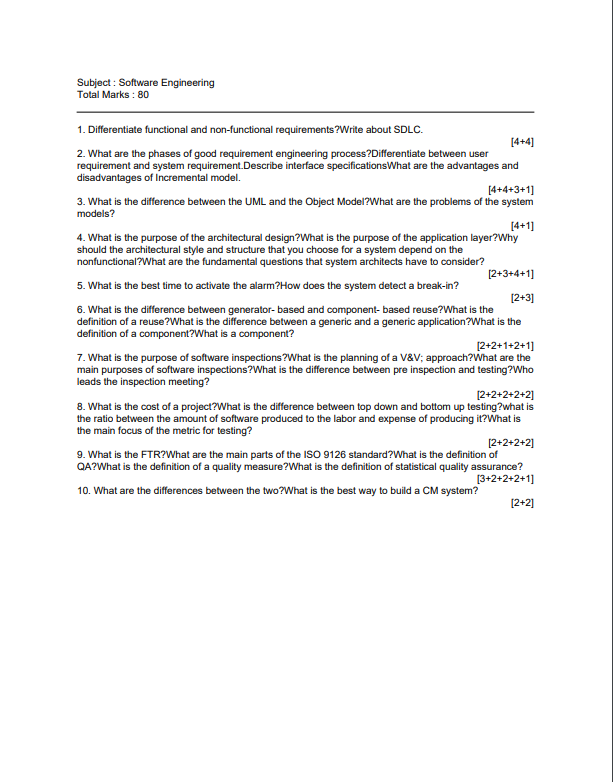
\includegraphics[scale = 1]{Images/generatedQuestionSet1.png}
    \captionsetup{justification=centering} 
    \caption{Result: Sample Question Set in PDF form}
\end{figure}
\section{Sample Question Set}
\pagebreak
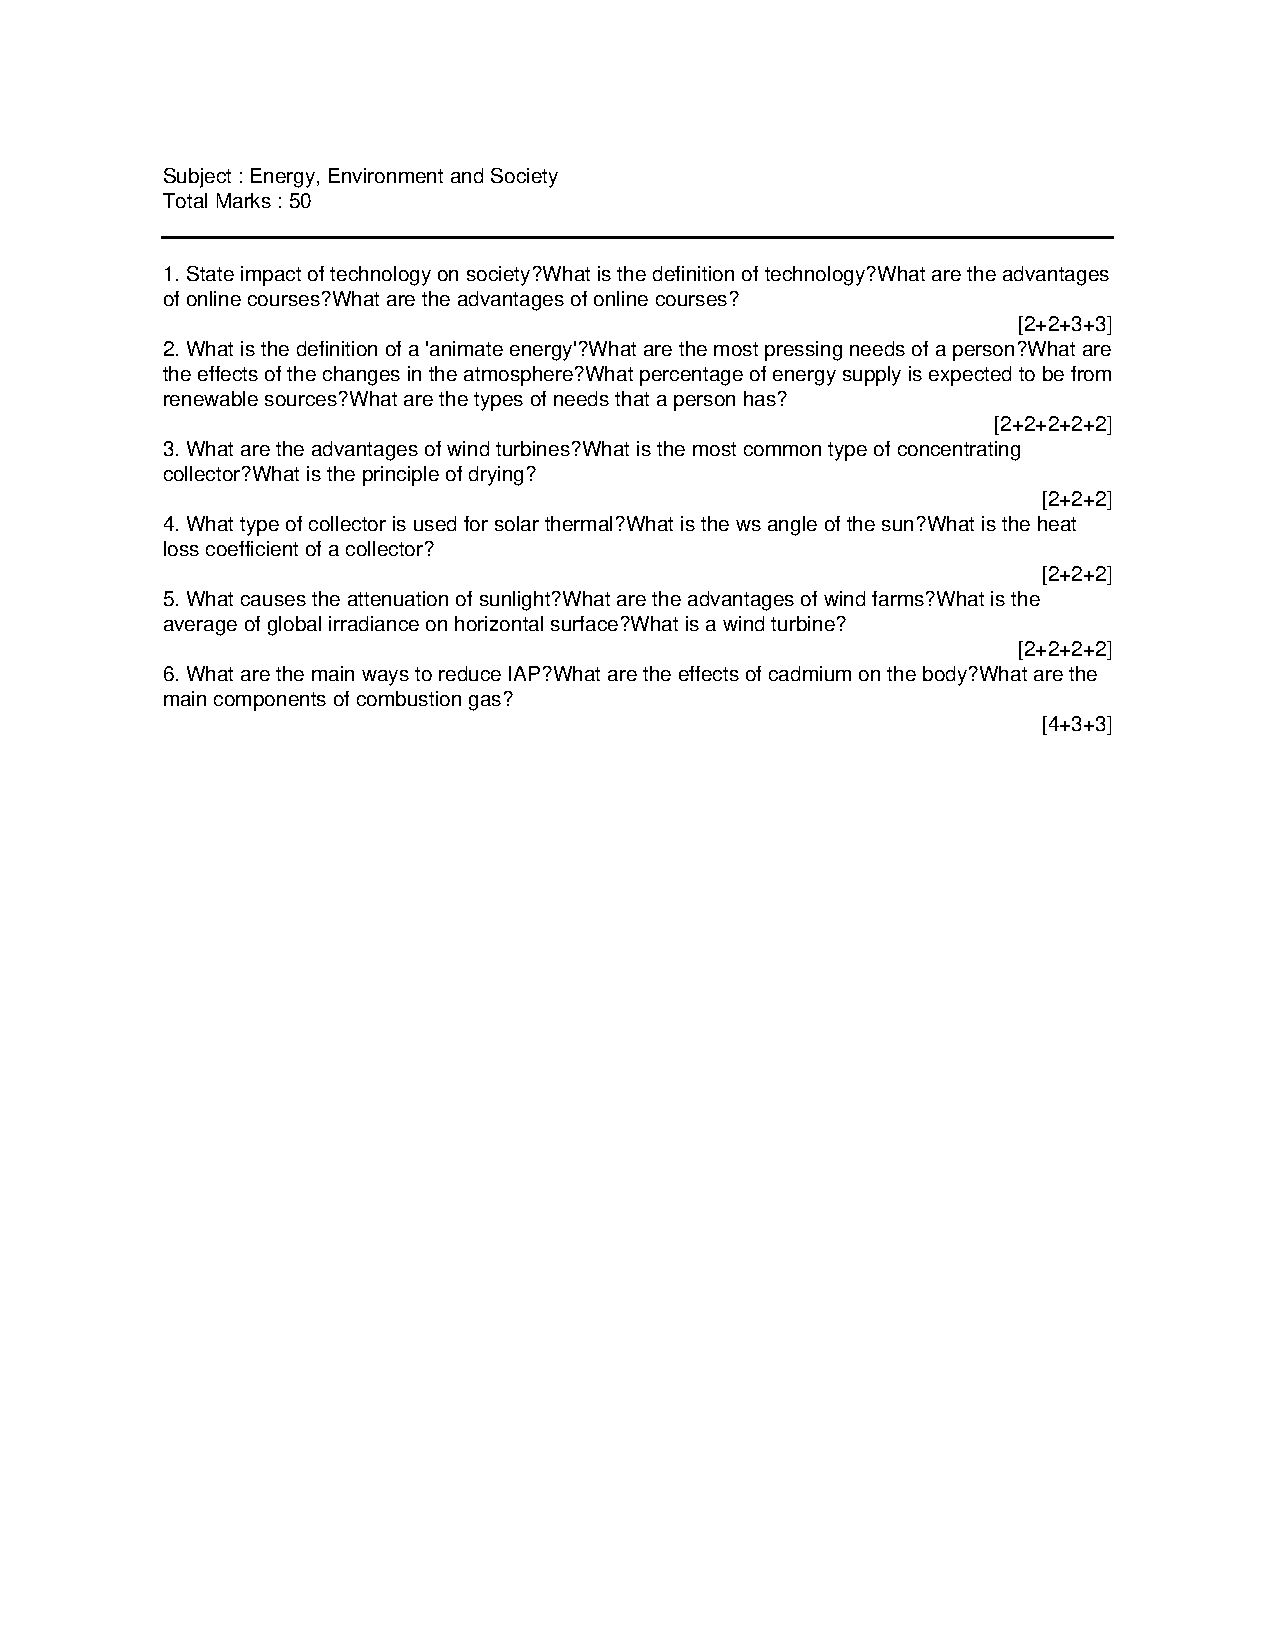
\includepdf[pages=-]{samples/EES.pdf}
\end{document}

